\documentclass[11pt]{article}

\usepackage[margin=1.2in]{geometry}
\usepackage{amsmath,amssymb}
\usepackage[T1]{fontenc}
\usepackage[utf8]{inputenc}
\usepackage{lmodern}
\usepackage{microtype}
\usepackage{booktabs}
\usepackage[hidelinks]{hyperref}
\usepackage{parskip}
\usepackage{enumitem}
\usepackage{tikz}
\usepackage[dvipsnames]{xcolor}
\usetikzlibrary{positioning, shapes.geometric, decorations.pathmorphing, arrows.meta, calc, patterns}
\usepackage{tcolorbox}
\newtcolorbox{keymessage}{%
  colback=blue!3, colframe=blue!40!black,
  fonttitle=\bfseries\small, title=Key Message,
  boxrule=0.5pt, arc=2pt, left=6pt, right=6pt, top=4pt, bottom=4pt
}

\title{The Map and the Territory:\\
A Constructive History of Mathematical Physics}
\author{Paul Chun-Kit Lee\\[2pt]
\small New York University}
\date{February 2026}

\begin{document}
\maketitle

\begin{abstract}
This essay tells the story of 150~years of mathematical physics from an unfamiliar angle.
A machine-verified research program---approximately 18,500~lines of formally checked proofs in the Lean~4 proof assistant---has established that every empirical prediction of quantum and statistical mechanics examined so far can be derived using only the most elementary constructive logic, without the law of excluded middle or any principle of omniscience.
The elaborate classical superstructure of modern physics---infinite-dimensional Hilbert spaces, thermodynamic limits, path integrals, singularity theorems---enters only through idealizations that no finite laboratory can instantiate.
The resulting hierarchy of logical strength is a partial order, not a chain: three independent branches (Dependent Choice, Markov's Principle, and the omniscience spine BISH~$<$~LLPO~$<$~WLPO~$<$~LPO) meet at the Fan Theorem in a fourth direction, and the logical cost of each idealization depends on the observable being computed, not merely the physical system under study.
This essay traces how classical logic was progressively imported into mathematical physics from the 1870s onward, what it cost at each stage, what constructive alternatives existed or could have been used instead, and what the pattern implies for the current state of theoretical physics.
This is Paper~12 in the Constructive Calibration Programme, a companion to the formal synthesis (Paper~10) \cite{Lee2026paper10}, written for a broader audience.
\end{abstract}

% ============================================================
\section{The Cellar and the Cathedral}
% ============================================================

The most precise prediction in the history of science is a number: the anomalous magnetic moment of the electron, usually called $g{-}2$.
Quantum electrodynamics predicts this quantity to roughly twelve decimal places, and experiment confirms it.
The agreement is so exact that if you measured the distance from New York to Los Angeles to the same relative precision, you would be accurate to the width of a human hair.

Here is the quiet scandal behind that triumph.
Every step of the actual computation is finite arithmetic.
A physicist draws a Feynman diagram---a small picture of particles interacting---and translates it into a definite integral over a finite number of momentum variables.
She evaluates the integral numerically, adds contributions from a finite number of diagrams at each level of approximation, and arrives at a rational number with controlled error bars.
Every operation could be performed by a mechanical calculator given enough time.
There is no step that requires surveying an infinite set, deciding an undecidable question, or asserting the existence of a completed infinite object.

And yet the formalism in which this computation is embedded is a cathedral of infinities.
The path integral---the foundational tool of quantum field theory---is, in its continuum formulation, an ``integral'' over an infinite-dimensional space of field configurations for which no mathematically rigorous measure exists in general.
(Euclidean lattice path integrals---Wilson's 1974 construction \cite{Wilson1974}---are mathematically rigorous but operate on finite lattices, i.e., at BISH.)
Fock space, the mathematical arena for multi-particle quantum mechanics, is an infinite-dimensional tensor product.
Renormalization, the procedure that extracts finite predictions from divergent expressions, involves manipulations with quantities that are formally infinite.
The vacuum state---the ``empty'' starting point of every calculation---is a vector in an infinite-dimensional space whose properties encode the entire structure of the theory.

\begin{figure}[ht]
\centering
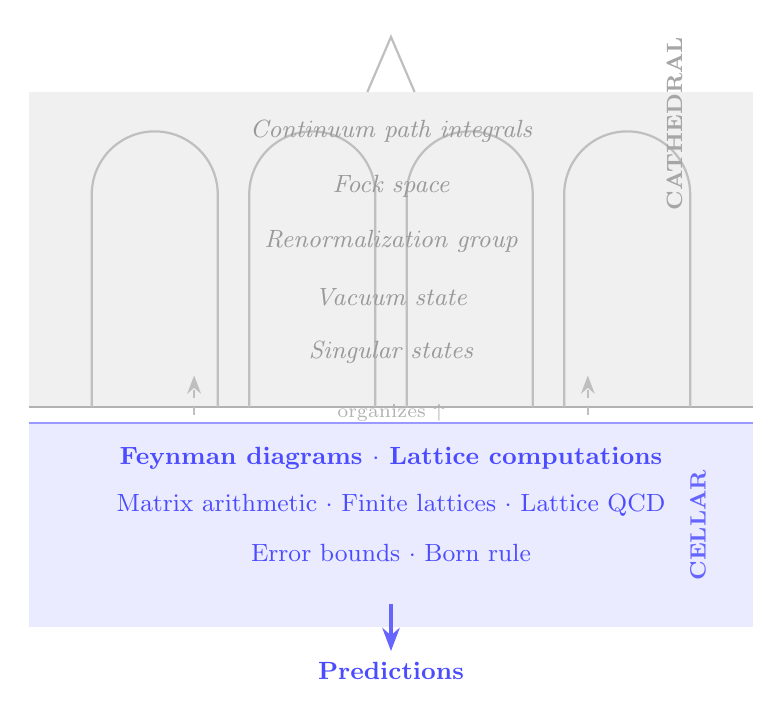
\begin{tikzpicture}[
  >=Stealth,
  every node/.style={font=\small}
]
% Cathedral (upper level) — shaded gray
\fill[gray!12] (-4.6, 2.8) rectangle (4.6, 6.8);
\draw[thick, gray!60] (-4.6, 2.8) -- (4.6, 2.8);
% Arches
\foreach \x in {-3, -1, 1, 3} {
  \draw[gray!50, thick] (\x-0.8, 2.8) -- (\x-0.8, 5.5) arc (180:0:0.8) -- (\x+0.8, 2.8);
}
% Spire
\draw[gray!50, thick] (-0.3, 6.8) -- (0, 7.5) -- (0.3, 6.8);
% Cathedral labels
\node[font=\small\itshape, gray!80] at (0, 6.3) {Continuum path integrals};
\node[font=\small\itshape, gray!80] at (0, 5.6) {Fock space};
\node[font=\small\itshape, gray!80] at (0, 4.9) {Renormalization group};
\node[font=\small\itshape, gray!80] at (0, 4.2) {Vacuum state};
\node[font=\small\itshape, gray!80] at (0, 3.5) {Singular states};
\node[font=\footnotesize\bfseries, gray!70] at (3.6, 6.4) {\rotatebox{90}{CATHEDRAL}};

% Cellar (lower level) — shaded blue
\fill[blue!8] (-4.6, 0) rectangle (4.6, 2.6);
\draw[thick, blue!40] (-4.6, 2.6) -- (4.6, 2.6);
% Cellar labels
\node[font=\small\bfseries, blue!70] at (0, 2.15) {Feynman diagrams $\cdot$ Lattice computations};
\node[font=\small, blue!70] at (0, 1.55) {Matrix arithmetic $\cdot$ Finite lattices $\cdot$ Lattice QCD};
\node[font=\small, blue!70] at (0, 0.95) {Error bounds $\cdot$ Born rule};
\node[font=\footnotesize\bfseries, blue!60] at (3.9, 1.3) {\rotatebox{90}{CELLAR}};

% Arrow: predictions flow up
\draw[->, very thick, blue!60] (0, 0.3) -- (0, -0.3) node[below, font=\small\bfseries, blue!70] {Predictions};

% Arrow: formalism sits above
\draw[->, thick, gray!50, dashed] (-2.5, 2.7) -- (-2.5, 3.2);
\draw[->, thick, gray!50, dashed] (2.5, 2.7) -- (2.5, 3.2);
\node[font=\scriptsize, gray!60] at (0, 2.73) {organizes $\uparrow$};

\end{tikzpicture}
\caption{The cellar and the cathedral. Every empirical prediction of quantum field theory (below) is a finite computation---BISH. The infinite-dimensional formalism (above) organizes the computations but is not itself physically instantiated.}
\label{fig:cellar-cathedral}
\end{figure}

The predictions come from the cellar.
The cathedral sits above: beautiful, architecturally magnificent, and largely empty.
Almost nobody computes a continuum path integral; in perturbative QFT, they compute Feynman diagrams, and in lattice QCD, they evaluate discretized path integrals on finite lattices---both BISH operations.
Nobody works in Fock space; they work with definite, finite numbers of particles.
The infinite-dimensional superstructure is a mnemonic---a way of organizing the finite computations---but the physics, the part that touches experiment, lives in the finite arithmetic below (Figure~\ref{fig:cellar-cathedral}).

This essay is about the gap between the cellar and the cathedral.
It is about the question: how much of the mathematical apparatus of physics describes the physical world, and how much describes the mathematician's toolkit?
For the first time, a machine-verified research program can answer this question with mathematical precision.
The answer is surprising, and it reaches back 150~years.
Every empirical prediction we have examined---across quantum mechanics, statistical mechanics, and general relativity---lives at the most elementary level of constructive logic.
The classical superstructure, with its completed infinities and its implicit appeals to omniscience over infinite sets, is the mapmaker's convention.
Nature, it appears, speaks a simpler language.

A word of framing before we proceed.
The map is not useless---it is an extraordinarily effective organizing tool.
Classical mathematics has powered the greatest quantitative achievements in the history of science.
But the map is not the territory.
The thesis of this essay is not that the classical formalism is wrong, but that it contains more structure than the physics requires, and that the excess structure has gradually been mistaken for reality.
The constructive hierarchy provides a precise tool for separating the territory from the mapmaker's conventions.

\begin{keymessage}
Every empirical prediction of QFT examined in this programme is finite arithmetic --- constructive analysis at BISH.
The infinite-dimensional formalism organizes computations but is not physically instantiated.
The predictions come from the cellar; the cathedral is the mathematician's convenience.
\end{keymessage}

A scope note: the calibration programme examines quantum states, static structures, and specific exactly solvable models---not quantum dynamics.
Time evolution, scattering amplitudes, the S-matrix, and real-time path integrals remain uncalibrated.
``BISH'' throughout this essay means Bishop-style constructive analysis---which includes real-valued computation with explicit moduli of convergence, not merely discrete or finite arithmetic.
The claims about empirical predictions should be read with both limitations in mind.


% ============================================================
\section{What Physicists Don't Know They're Assuming}
% ============================================================

To understand what the research program has discovered, you need to understand a distinction that most physicists have never encountered: the difference between levels of \emph{logical strength} in mathematics.

Before describing the hierarchy, a crucial clarification.
The hierarchy of logical strength (BISH $<$ WLPO $<$ LPO $<$ LEM) measures what \emph{principles} a proof requires---what kind of assertions about infinite sets you must accept.
This is entirely different from Turing undecidability, which measures what no \emph{algorithm} can compute regardless of the axioms you accept.
A problem can be Turing-decidable yet require LPO to prove (the thermodynamic limit), or Turing-undecidable yet live outside the omniscience hierarchy entirely (the spectral gap problem of Cubitt et~al.\ \cite{Cubitt2015}, which is Turing-undecidable).
The spectral gap is undecidable in the sense that no algorithm can determine the answer from a Hamiltonian's local rules; this is not ``a level above LEM'' in the logical hierarchy but an orthogonal phenomenon.
Throughout this essay, ``logical strength'' refers to the constructive hierarchy, not to computability in the Turing sense.

Consider an infinite hotel with rooms numbered 1, 2, 3, and so on.
You want to know whether every room is empty.
Here are four different things you might be allowed to assert, each representing a different level of logical power.

At the first level---call it \textbf{BISH}, for Bishop-style constructive mathematics \cite{Bishop1967}---you can check rooms one by one, and you can report what you find.
If you have a proof that works for every room (a master key, say, that shows no guest could possibly be registered), you may declare ``all empty.''
If you find an occupied room, you may point to it and say ``room 47 is occupied.''
But you may \emph{not} declare ``they're all empty'' without a universal proof, and you may not declare ``someone's home'' without producing the room number.
You claim only what you can demonstrate.

At the second level---\textbf{WLPO}, the Weak Limited Principle of Omniscience---you gain a modest superpower.
You may assert either ``all rooms are empty'' \emph{or} ``it is not the case that all rooms are empty.''
But in the second case, you do not need to produce the occupied room.
You know something is there; you just cannot point to it.

At the third level---\textbf{LPO}, the Limited Principle of Omniscience---you have full dichotomy.
Either ``all rooms are empty'' or ``here is the occupied room.''
No ambiguity, no gap between knowing something exists and finding it.

At the fourth level---\textbf{LEM}, the Law of Excluded Middle, which is the logic of standard mathematics---you can answer \emph{any} yes-or-no question about the hotel instantly.
Not just occupancy: any question whatsoever, about any collection of mathematical objects, has a definite true-or-false answer, whether or not you can determine which.

Between WLPO and LPO lie two further levels that the research programme has now populated with physical content.
At \textbf{LLPO}, the Lesser Limited Principle of Omniscience, you can determine the \emph{sign} of a nonzero quantity---``this is positive or this is negative''---without the full dichotomy of LPO\@.
In the hotel metaphor, you know the occupied rooms are all on even floors or all on odd floors, but you cannot point to a specific room.
LLPO is strictly between WLPO and LPO\@.
Separately, the \textbf{Fan Theorem} (FT) asserts that a pointwise property of all infinite paths through a finitely branching tree can be witnessed by a uniform finite bound.
FT is independent of the entire omniscience spine---it neither implies nor is implied by LPO---and occupies a distinct branch of the partial order.
In the hotel metaphor, FT says: if every guest checks out eventually, there is a uniform checkout time that works for all of them, without needing to know which room each guest occupied.

These levels form a partial order, not a simple chain: BISH is the weakest, LEM is the strongest, but there are independent branches (DC$_\omega$, MP, FT) that neither imply each other nor imply WLPO \cite{BridgesVita2006, BridgesRichman1987}.
The separations are strict---there are mathematical universes where WLPO holds but LPO fails, where LLPO holds but WLPO fails, and where FT holds but LPO fails.

The hierarchy is not esoteric.
Each step up the ladder is a specific claim about your ability to decide questions involving infinite collections.
BISH says: decide only what you can verify by a finite procedure.
LLPO says: you may determine the sign of a nonzero real.
WLPO says: you may know that something is true ``in principle'' without exhibiting a witness.
LPO says: you may decide existence claims about infinite sequences.
FT says: pointwise finiteness implies uniform finiteness.
LEM says: everything is decidable, period.

\begin{figure}[ht]
\centering
\resizebox{\textwidth}{!}{%
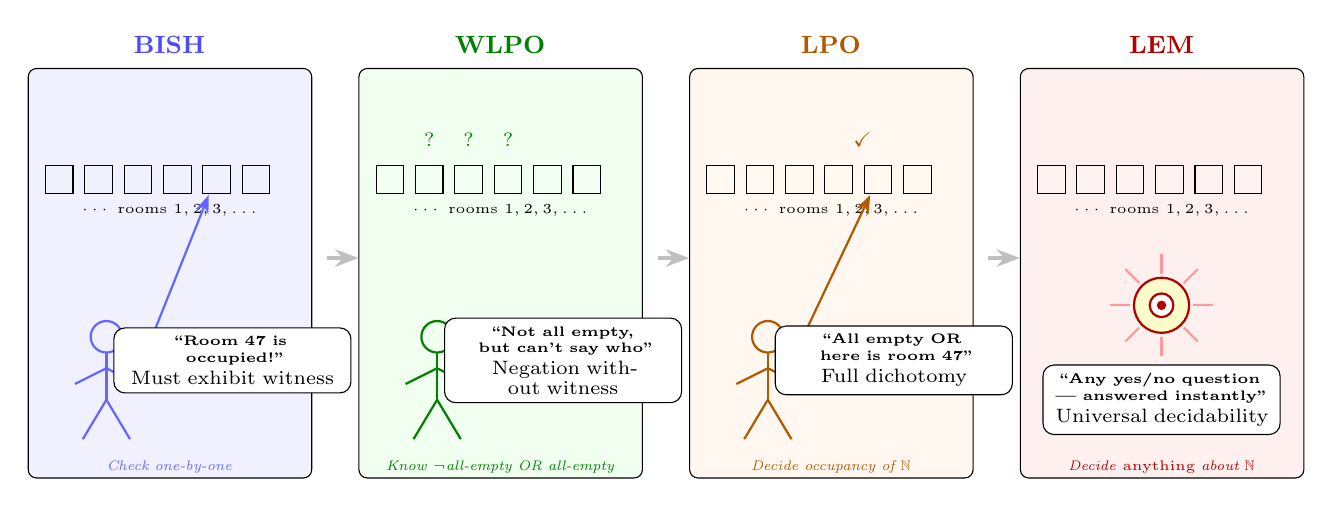
\begin{tikzpicture}[
  >=Stealth,
  panel/.style={draw, rounded corners=3pt, minimum width=3.6cm, minimum height=5.2cm, anchor=south west},
  roomstyle/.style={draw, minimum width=0.35cm, minimum height=0.35cm, inner sep=0pt},
  bubble/.style={draw, rounded corners=4pt, fill=white, font=\tiny, text width=2.8cm, align=center, inner sep=3pt}
]
% Panel 1: BISH
\node[panel, fill=blue!6] (p1) at (0,0) {};
\node[font=\small\bfseries, blue!70] at (1.8, 5.5) {BISH};
% Hotel rooms
\foreach \i in {0,...,5} {
  \node[roomstyle, fill=blue!5] at (0.4+\i*0.5, 3.8) {};
}
\node[font=\tiny] at (1.8, 3.4) {$\cdots$ rooms $1, 2, 3, \ldots$};
% Stick figure checking rooms
\draw[thick, blue!60] (1.0, 1.8) circle (0.2);
\draw[thick, blue!60] (1.0, 1.6) -- (1.0, 1.0);
\draw[thick, blue!60] (1.0, 1.4) -- (0.6, 1.2);
\draw[thick, blue!60] (1.0, 1.4) -- (1.4, 1.2);
\draw[thick, blue!60] (1.0, 1.0) -- (0.7, 0.5);
\draw[thick, blue!60] (1.0, 1.0) -- (1.3, 0.5);
% Arrow pointing to room
\draw[->, thick, blue!60] (1.5, 1.6) -- (2.3, 3.6);
% Speech bubble
\node[bubble] at (2.6, 1.5) {\textbf{``Room 47 is\\occupied!''}\\[2pt]\scriptsize Must exhibit witness};
\node[font=\tiny\itshape, blue!60] at (1.8, 0.15) {Check one-by-one};

% Panel 2: WLPO
\node[panel, fill=green!6] (p2) at (4.2,0) {};
\node[font=\small\bfseries, green!50!black] at (6.0, 5.5) {WLPO};
\foreach \i in {0,...,5} {
  \node[roomstyle, fill=green!5] at (4.6+\i*0.5, 3.8) {};
}
\node[font=\tiny] at (6.0, 3.4) {$\cdots$ rooms $1, 2, 3, \ldots$};
% Stick figure at desk
\draw[thick, green!50!black] (5.2, 1.8) circle (0.2);
\draw[thick, green!50!black] (5.2, 1.6) -- (5.2, 1.0);
\draw[thick, green!50!black] (5.2, 1.4) -- (4.8, 1.2);
\draw[thick, green!50!black] (5.2, 1.4) -- (5.6, 1.2);
\draw[thick, green!50!black] (5.2, 1.0) -- (4.9, 0.5);
\draw[thick, green!50!black] (5.2, 1.0) -- (5.5, 0.5);
% Question marks over rooms
\node[font=\scriptsize, green!50!black] at (5.1, 4.3) {?};
\node[font=\scriptsize, green!50!black] at (5.6, 4.3) {?};
\node[font=\scriptsize, green!50!black] at (6.1, 4.3) {?};
% Speech bubble
\node[bubble] at (6.8, 1.5) {\textbf{``Not all empty,\\but can't say who''}\\[2pt]\scriptsize Negation without witness};
\node[font=\tiny\itshape, green!50!black] at (6.0, 0.15) {Know $\lnot$all-empty OR all-empty};

% Panel 3: LPO
\node[panel, fill=orange!6] (p3) at (8.4,0) {};
\node[font=\small\bfseries, orange!70!black] at (10.2, 5.5) {LPO};
\foreach \i in {0,...,5} {
  \node[roomstyle, fill=orange!5] at (8.8+\i*0.5, 3.8) {};
}
\node[font=\tiny] at (10.2, 3.4) {$\cdots$ rooms $1, 2, 3, \ldots$};
% Oracle figure
\draw[thick, orange!70!black] (9.4, 1.8) circle (0.2);
\draw[thick, orange!70!black] (9.4, 1.6) -- (9.4, 1.0);
\draw[thick, orange!70!black] (9.4, 1.4) -- (9.0, 1.2);
\draw[thick, orange!70!black] (9.4, 1.4) -- (9.8, 1.2);
\draw[thick, orange!70!black] (9.4, 1.0) -- (9.1, 0.5);
\draw[thick, orange!70!black] (9.4, 1.0) -- (9.7, 0.5);
% Check mark and arrow
\draw[->, thick, orange!70!black] (9.8, 1.7) -- (10.7, 3.6);
\node[font=\scriptsize, orange!70!black] at (10.6, 4.3) {\checkmark};
% Speech bubble
\node[bubble] at (11.0, 1.5) {\textbf{``All empty OR\\here is room 47''}\\[2pt]\scriptsize Full dichotomy};
\node[font=\tiny\itshape, orange!70!black] at (10.2, 0.15) {Decide occupancy of $\mathbb{N}$};

% Panel 4: LEM
\node[panel, fill=red!6] (p4) at (12.6,0) {};
\node[font=\small\bfseries, red!70!black] at (14.4, 5.5) {LEM};
\foreach \i in {0,...,5} {
  \node[roomstyle, fill=red!5] at (13.0+\i*0.5, 3.8) {};
}
\node[font=\tiny] at (14.4, 3.4) {$\cdots$ rooms $1, 2, 3, \ldots$};
% God's eye
\draw[thick, red!70!black, fill=yellow!20] (14.4, 2.2) circle (0.35);
\draw[thick, red!70!black, fill=white] (14.4, 2.2) circle (0.15);
\fill[red!70!black] (14.4, 2.2) circle (0.06);
% Rays
\foreach \a in {0,45,...,315} {
  \draw[red!40, thick] (14.4, 2.2) ++ (\a:0.4) -- ++ (\a:0.25);
}
% Speech bubble
\node[bubble] at (14.4, 1.0) {\textbf{``Any yes/no question\\--- answered instantly''}\\[2pt]\scriptsize Universal decidability};
\node[font=\tiny\itshape, red!70!black] at (14.4, 0.15) {Decide \emph{anything} about $\mathbb{N}$};

% Arrows showing hierarchy
\draw[->, very thick, gray!50] (3.8, 2.8) -- (4.2, 2.8);
\draw[->, very thick, gray!50] (8.0, 2.8) -- (8.4, 2.8);
\draw[->, very thick, gray!50] (12.2, 2.8) -- (12.6, 2.8);

\end{tikzpicture}%
}% end resizebox
\caption{The infinite hotel at four logical levels.
\textbf{BISH}: you may assert only what you can verify by finite procedure.
\textbf{WLPO}: you may assert ``not all empty'' without producing the occupied room.
\textbf{LPO}: full dichotomy on infinite sequences---either all empty or exhibit a witness.
\textbf{LEM}: every yes/no question about any mathematical object has a definite answer.
Each level implies all those to its left; the implications are strict.}
\label{fig:hotel}
\end{figure}

Physicists work at the top of this ladder without a second thought.
Every proof in a standard textbook uses the law of excluded middle freely: a particle is either in this region or it isn't; a sequence either converges or it doesn't; a geodesic either terminates or it extends forever.
The question this essay addresses is whether the physics \emph{needs} all that logical power, or whether the predictions would survive with less.

Think of it this way.
Every theorem in a physics textbook has an invisible footnote reading: ``This proof also assumes that you can survey infinite sets in a single glance.''
The research program described here identifies which theorems genuinely need that footnote and which would stand without it.

\begin{figure}[ht]
\centering
\resizebox{\textwidth}{!}{%
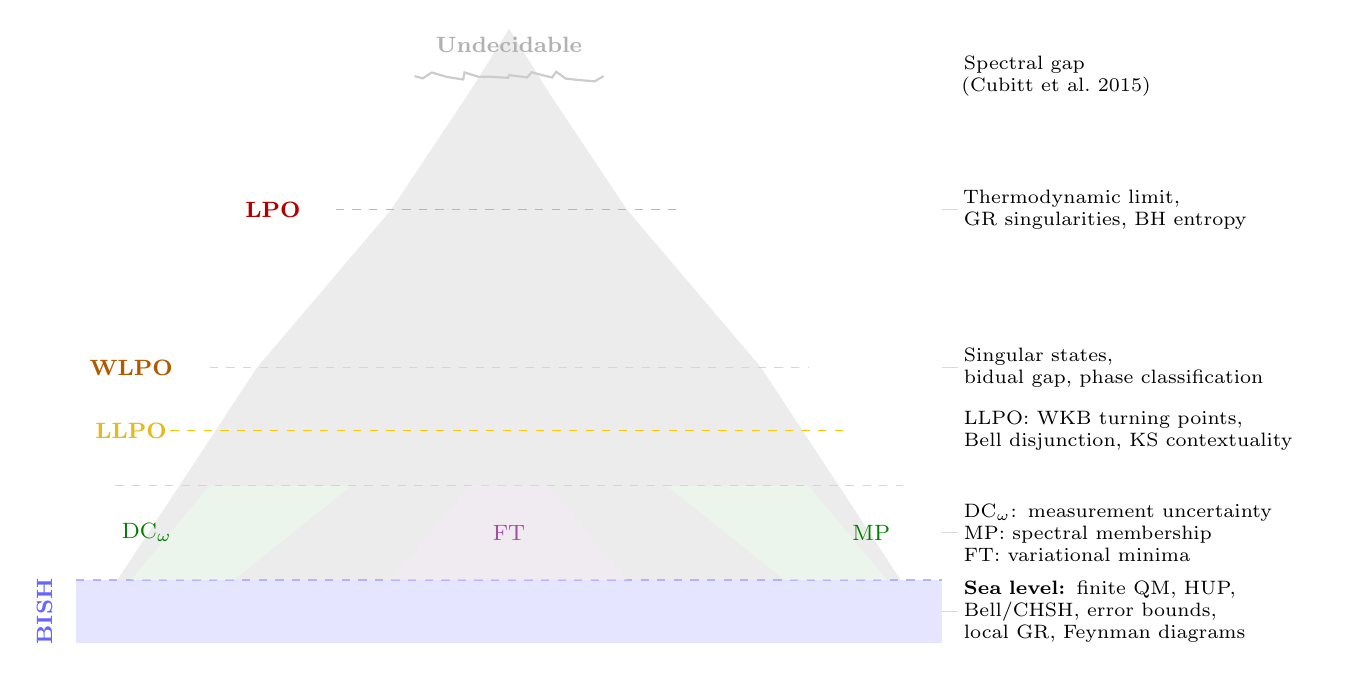
\begin{tikzpicture}[
  >=Stealth,
  every node/.style={font=\small},
  physlabel/.style={font=\scriptsize, text width=4.5cm, align=left, inner sep=2pt}
]
% Mountain body
\fill[gray!15] (-5.5,0) -- (-3.2, 3.5) -- (-1.5, 5.5) -- (-0.5, 7.0) -- (0, 7.8) -- (0.5, 7.0) -- (1.5, 5.5) -- (3.2, 3.5) -- (5.5, 0) -- cycle;
% Altitude bands — shaded
\fill[blue!10] (-5.5, 0) -- (-5.5, 0.8) -- (5.5, 0.8) -- (5.5, 0) -- cycle;
\draw[blue!30, dashed] (-5.5, 0.8) -- (5.5, 0.8);
% Sea level label
\node[font=\footnotesize\bfseries, blue!60] at (-5.9, 0.4) {\rotatebox{90}{BISH}};
% Foothills
\fill[green!8, opacity=0.5] (-4.8, 0.8) -- (-3.8, 2.0) -- (-2.0, 2.0) -- (-3.5, 0.8) -- cycle;
\fill[green!8, opacity=0.5] (3.5, 0.8) -- (2.0, 2.0) -- (3.8, 2.0) -- (4.8, 0.8) -- cycle;
\draw[green!40, dashed] (-5.0, 2.0) -- (5.0, 2.0);
\node[font=\footnotesize, green!50!black] at (-4.6, 1.4) {\footnotesize DC$_\omega$};
\node[font=\footnotesize, green!50!black] at (4.6, 1.4) {\footnotesize MP};
% LLPO ledge
\draw[yellow!60!orange, dashed] (-4.3, 2.7) -- (4.3, 2.7);
\node[font=\footnotesize\bfseries, yellow!60!orange!90!black] at (-4.8, 2.7) {LLPO};
% FT foothill (independent branch)
\fill[violet!8, opacity=0.5] (-1.5, 0.8) -- (-0.5, 2.0) -- (0.5, 2.0) -- (1.5, 0.8) -- cycle;
\node[font=\footnotesize, violet!70] at (0, 1.4) {\footnotesize FT};
% Mountainside
\draw[orange!40, dashed] (-3.8, 3.5) -- (3.8, 3.5);
\node[font=\footnotesize\bfseries, orange!70!black] at (-4.8, 3.5) {WLPO};
% Summit
\draw[red!40, dashed] (-2.2, 5.5) -- (2.2, 5.5);
\node[font=\footnotesize\bfseries, red!70!black] at (-3.0, 5.5) {LPO};
% Cloud at top
\draw[gray!40, thick, decorate, decoration={random steps, segment length=4pt, amplitude=2pt}]
  (-1.2, 7.2) -- (1.2, 7.2);
\node[font=\footnotesize\bfseries, gray!60] at (0, 7.6) {Undecidable};

% Physics labels on right
\node[physlabel, anchor=west] at (5.7, 0.4)
  {\textbf{Sea level:} finite QM, HUP,\\Bell/CHSH, error bounds,\\local GR, Feynman diagrams};
\node[physlabel, anchor=west] at (5.7, 1.4)
  {DC$_\omega$: measurement uncertainty\\MP: spectral membership\\FT: variational minima};
\node[physlabel, anchor=west] at (5.7, 2.7)
  {LLPO: WKB turning points,\\Bell disjunction, KS contextuality};
\node[physlabel, anchor=west] at (5.7, 3.5)
  {Singular states,\\bidual gap, phase classification};
\node[physlabel, anchor=west] at (5.7, 5.5)
  {Thermodynamic limit,\\GR singularities, BH entropy};
\node[physlabel, anchor=west] at (5.7, 7.2)
  {Spectral gap\\(Cubitt et al.\ 2015)};

% Connecting lines
\foreach \y/\xr in {0.4/5.5, 1.4/5.5, 3.5/5.5, 5.5/5.5} {
  \draw[gray!30, thin] (5.5, \y) -- (\xr+0.2, \y);
}

\end{tikzpicture}%
}% end resizebox
\caption{The logical geography of mathematical physics, depicted as a mountain.
Sea level (BISH) contains all empirical predictions. Higher altitudes correspond to
greater logical strength---stronger principles, not greater computational complexity.
DC$_\omega$, MP, and FT occupy independent foothills---none implies any other, and none
implies WLPO\@.
LLPO occupies a ledge between the foothills and the mountainside.
The summit (LPO) contains the thermodynamic limit, singularity theorems, and BH entropy convergence.
Beyond it lies Turing undecidability, which is orthogonal to the logical-strength hierarchy.}
\label{fig:mountain}
\end{figure}

To give the hierarchy a visual anchor, imagine a mountain (Figure~\ref{fig:mountain}).
Sea level is BISH---constructive mathematics, finite procedures, the logic of computation.
The foothills are occupied by Dependent Choice, Markov's Principle, and the Fan Theorem---modest extensions that allow countable sequences of choices, conclude existence from the impossibility of non-existence, or extract uniform bounds from pointwise data.
These three foothills are \emph{independent}: none implies any other, and none implies WLPO.
The mountain has ridges running in different directions.
A ledge at LLPO---the Lesser Limited Principle of Omniscience---sits between the foothills and the mountainside.
LLPO governs sign decisions: it lets you determine whether a nonzero quantity is positive or negative without the full witness that LPO provides.
Physically, it is the cost of asserting that a general continuous potential has classical turning points (WKB, Paper~19) and the cost of the disjunction in Bell's theorem (Paper~21) and Kochen-Specker contextuality (Paper~24).
The mountainside is WLPO---where infinite-dimensional analysis begins to part company with finite approximation.
The summit is LPO---the regime of completed infinite limits, thermodynamic idealization, and the convergence of bounded monotone sequences.
Beyond the summit, the air is too thin for any consistent formal system: the spectral gap problem \cite{Cubitt2015} lives here, undecidable in principle.

The topology of this mountain is richer than a simple linear chain.
The hierarchy is a \emph{partial order}: BISH $<$ LLPO $<$ WLPO $<$ LPO forms the omniscience spine, but DC$_\omega$, MP, and FT branch off independently from BISH, creating a tree with at least four upward paths from sea level.
Different physical idealizations draw on different branches: the Born rule's infinite-ensemble convergence requires DC$_\omega$; exact spectral membership requires MP; variational ground-state existence requires FT; sign decisions in quantum tunnelling require LLPO.
No single chain captures the full structure.
The logical geography of physics is, fittingly, a landscape with multiple ridges.

The research program maps the major theorems of mathematical physics onto this mountain.
The results are striking.
Everything a laboratory does---every preparation, every measurement, every finite computation---lives at sea level.
The idealizations begin on the mountainside, and the summit is populated exclusively by objects that no experiment can instantiate.

\begin{keymessage}
Mathematical physics uses a partial order of logical strength: the omniscience spine BISH $<$ LLPO $<$ WLPO $<$ LPO, with independent branches DC$_\omega$, MP, and FT\@.
Every laboratory operation lives at sea level (BISH).
The question this essay addresses is whether the physics needs the higher altitudes.
\end{keymessage}

% ============================================================
\section{Act~I: The Weierstrass Inheritance (1870--1900)}
% ============================================================

The story begins not with physics but with mathematics.

Before Weierstrass, mathematicians computed with infinitesimals---entities that were simultaneously zero and not zero, useful for deriving results but philosophically disreputable.
In the 1860s and 1870s, Weierstrass and his contemporaries replaced infinitesimals with the epsilon-delta formalism: a limit is not a process of ``approaching'' but a statement about the existence of real numbers satisfying certain inequalities.
This was a triumph of rigor.
It eliminated hand-waving, made proofs precise, and gave calculus a foundation that could withstand logical scrutiny.

But the foundation came with hidden freight.
The completeness of the real numbers---the assertion that every bounded increasing sequence of rationals converges to a definite real number---is not a free theorem.
In constructive mathematics, bounded monotone convergence is equivalent to LPO \cite{BridgesVita2006}.
To assert that a bounded monotone sequence converges, you must assert a dichotomy on an infinite object: either the sequence stabilizes or a witness to non-stabilization can be produced.
Weierstrass imported LPO into the foundations of analysis, and physicists inherited it without noticing.

The physical consequences arrived with Boltzmann.
Statistical mechanics, as developed by Boltzmann and Gibbs in the 1870s through 1900s, introduced the thermodynamic limit: take a system of $N$ particles, let $N \to \infty$, and define temperature, entropy, and free energy as properties of the infinite system.
The motivation was practical---you cannot track $10^{23}$ particles individually---but the mathematical move was fateful.
The free energy per particle, $f(\beta) = \lim_{N \to \infty} f_N(\beta)$, is defined as a completed limit.
Asserting that this limit \emph{exists as a definite real number} is equivalent to LPO \cite{Lee2026c}.

Our research program makes this precise.
For the one-dimensional Ising model---the simplest model of magnetism, a chain of interacting spins---the partition function is $Z_N = \operatorname{Tr}(T^N)$ where $T$ is a $2\times 2$ transfer matrix with constructively computable eigenvalues $\lambda_+ > \lambda_- > 0$.
The finite-size free energy $f_N(\beta)$ satisfies:
\begin{equation}\label{eq:ising-bound}
|f_N(\beta) - f_\infty(\beta)| \;\leq\; \frac{1}{N}\,\tanh(\beta J)^N,
\end{equation}
where $J$ is the coupling strength and $\beta$ is the inverse temperature.
This bound is provable in BISH---no omniscience principle required.
The geometric decay $\tanh(\beta J)^N$ is elementary, the eigenvalue computation is finite, and the error estimate is rational arithmetic with controlled precision.
The empirical content of the thermodynamic limit is available for free.
The difference is between ``for any desired precision, here is a finite system that achieves it'' (constructive) and ``there is a completed infinite-volume answer'' (LPO \cite{Lee2026c, Lee2026e}).

Phase transitions illustrate the stakes.
The standard account presents phase transitions---water freezing, magnets losing their magnetization at a critical temperature---as physical phenomena.
The mathematical account reveals that they are \emph{discontinuities in thermodynamic potentials}, and such discontinuities exist only in the infinite-volume limit.
Finite systems have smooth, analytic free energies; the discontinuity appears only when $N = \infty$.
In our framework, the discontinuity requires LPO; the physics it describes---the increasingly sharp feature in the free energy of large but finite systems---does not.

Boltzmann did not go astray, exactly.
The thermodynamic limit is an extraordinarily useful computational device.
But he introduced the first confusion between a mathematical convenience and a physical fact: the sharp phase transition, which exists only in the completed limit, was treated as a \emph{discovery about nature} rather than a \emph{property of the idealization}.
The thermodynamic limit is the map's convention that a coastline has a definite length.
The coastline doesn't know about the convention.

\textbf{The constructive alternative.}
It existed at the time.
Leopold Kronecker, Weierstrass's colleague and rival in Berlin, had advocated since the 1870s that mathematics should be restricted to finite constructions from natural numbers---essentially BISH before BISH existed.
His dictum, reported by Weber in 1893, captures the position: ``God made the integers; all else is the work of man.''
Kronecker directly opposed the completed reals and the Bolzano-Weierstrass theorem.
Moreover, Boltzmann's statistical mechanics was originally formulated for finite systems.
The passage to $N \to \infty$ was a later mathematical convenience, not a physical necessity.
Finite-system partition functions are constructively computable, and the error bound~\eqref{eq:ising-bound} shows that the empirical predictions of the infinite-volume theory are recoverable from finite data at BISH.
The constructive road was available from the start; the community took the other fork.

\begin{figure}[ht]
\centering
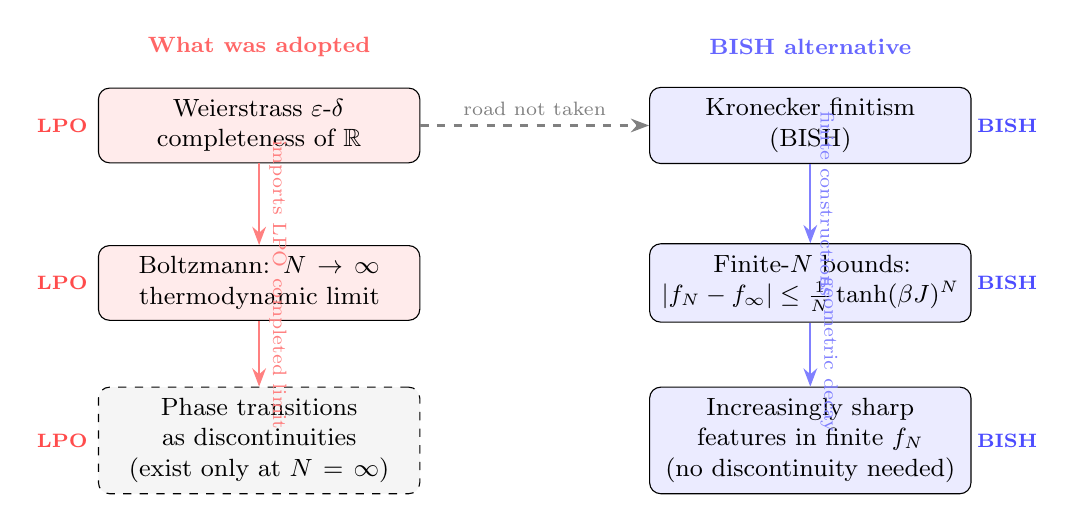
\begin{tikzpicture}[
  >=Stealth,
  every node/.style={font=\small},
  box/.style={draw, rounded corners, minimum height=0.9cm, text width=3.8cm, align=center, inner sep=4pt},
  adopted/.style={box, fill=red!8},
  bish/.style={box, fill=blue!8},
  result/.style={box, fill=gray!8, dashed},
  lbl/.style={font=\scriptsize, midway, above, sloped}
]
% Left column: what was adopted
\node[adopted] (weier) at (0, 4) {Weierstrass $\varepsilon$-$\delta$\\completeness of $\mathbb{R}$};
\node[adopted] (boltz) at (0, 2) {Boltzmann: $N \to \infty$\\thermodynamic limit};
\node[result] (phase) at (0, 0) {Phase transitions\\as discontinuities\\(exist only at $N = \infty$)};

% Right column: BISH alternative
\node[bish] (kron) at (7, 4) {Kronecker finitism\\(BISH)};
\node[bish] (finite) at (7, 2) {Finite-$N$ bounds:\\$|f_N - f_\infty| \leq \frac{1}{N}\tanh(\beta J)^N$};
\node[bish] (sharp) at (7, 0) {Increasingly sharp\\features in finite $f_N$\\(no discontinuity needed)};

% Arrows left column
\draw[->, thick, red!50] (weier) -- node[lbl] {imports LPO} (boltz);
\draw[->, thick, red!50] (boltz) -- node[lbl] {completed limit} (phase);

% Arrows right column
\draw[->, thick, blue!50] (kron) -- node[lbl] {finite constructions} (finite);
\draw[->, thick, blue!50] (finite) -- node[lbl] {geometric decay} (sharp);

% Cross arrows
\draw[->, thick, dashed, gray] (weier) -- node[above, font=\scriptsize] {road not taken} (kron);

% Labels
\node[font=\footnotesize\bfseries, red!60] at (0, 5) {What was adopted};
\node[font=\footnotesize\bfseries, blue!60] at (7, 5) {BISH alternative};

% Cost labels
\node[font=\scriptsize\bfseries, red!70] at (-2.5, 4) {LPO};
\node[font=\scriptsize\bfseries, red!70] at (-2.5, 2) {LPO};
\node[font=\scriptsize\bfseries, red!70] at (-2.5, 0) {LPO};
\node[font=\scriptsize\bfseries, blue!70] at (9.5, 4) {BISH};
\node[font=\scriptsize\bfseries, blue!70] at (9.5, 2) {BISH};
\node[font=\scriptsize\bfseries, blue!70] at (9.5, 0) {BISH};

\end{tikzpicture}
\caption{Act~I: the Weierstrass--Boltzmann import.
Weierstrass's completeness of the reals (LPO) was inherited by Boltzmann's thermodynamic limit.
The BISH alternative---finite-$N$ error bounds with geometric decay---recovers every empirical prediction without the completed limit.
The ``road not taken'' from Kronecker finitism was available from the 1870s.}
\label{fig:act1-import}
\end{figure}

% ============================================================
\section{Act~II: The Quantum Formalization (1925--1935)}
% ============================================================

Quantum mechanics was born constructive and became classical.

Heisenberg's matrix mechanics (1925) was intrinsically finite-dimensional and algebraic.
Matrices, commutators, trace formulas---the operational toolkit of quantum mechanics is linear algebra, and finite-dimensional linear algebra is BISH to the core.
Schr\"odinger's wave mechanics (1926) introduced infinite-dimensional function spaces, but the actual calculations---the hydrogen atom, the harmonic oscillator---used finite-term power series and explicit formulas.
Dirac's transformation theory (1927) unified matrix and wave mechanics through a powerful notation that also obscured the question of dimension.

A scope note is necessary here.
The constructive calibration programme examines quantum \emph{states}---density matrices, singular states, spectral structure---not quantum \emph{dynamics}.
Time evolution operators, scattering amplitudes, the S-matrix, and path integrals for dynamical processes remain uncalibrated.
The results below concern the static mathematical objects of quantum theory, not the dynamical ones.

Then came von~Neumann.

In 1932, von~Neumann published \emph{Mathematische Grundlagen der Quantenmechanik} \cite{vonNeumann1932}, which axiomatized quantum mechanics in terms of infinite-dimensional Hilbert spaces, the spectral theorem for unbounded self-adjoint operators, and the theory of von~Neumann algebras.
This was a masterwork of mathematical architecture.
It was also an act of mathematical imperialism: a finite, operational physical theory was recast in the language of infinite-dimensional functional analysis, and the physics community gradually lost the ability to distinguish the physics from the formalism.

Our program reveals the cost.
The Heisenberg uncertainty principle---arguably the defining statement of quantum mechanics---splits into two logically distinct results \cite{Lee2026g}.
The \emph{preparation uncertainty} inequality (the Robertson-Schr\"odinger bound) states that for any quantum state~$\psi$ with $\|\psi\|=1$ and any pair of observables $A$, $B$:
\begin{equation}\label{eq:rs-inequality}
|\langle \psi, [A,B]\,\psi\rangle|^2 \;\leq\; 4\,\mathrm{Var}_\psi(A)\;\mathrm{Var}_\psi(B),
\end{equation}
where $\mathrm{Var}_\psi(A) = \|A\psi - \langle A\rangle\psi\|^2$ and $[A,B] = AB - BA$.
This is fully constructive: the proof centers the state, applies the Cauchy-Schwarz inequality to the inner product $\langle \Delta_A\psi, \Delta_B\psi\rangle$, and decomposes the result into commutator and anticommutator contributions.
Pure Hilbert space geometry---BISH.
The \emph{measurement uncertainty} form---which concerns the statistics extracted from repeated measurements---requires Dependent Choice, a modest extension that allows countable sequences of dependent selections.
The physical core of quantum uncertainty needs no classical logic.
The classical overhead enters only when you extract statistical information from infinite measurement sequences.

This separation has a deeper significance than a technical footnote about choice principles.
The Born rule---the postulate that measurement probabilities equal $|\langle\lambda|\psi\rangle|^2$---is itself an idealization.
It asserts that relative frequencies over infinitely many measurements converge to definite probabilities; that convergence is where Dependent Choice enters.
The geometric content of quantum mechanics---that a single state cannot be simultaneously sharp in non-commuting observables---is BISH, a property of one vector in a finite-dimensional Hilbert space requiring no measurements at all.
The statistical content---that repeated measurements yield frequencies approaching the Born probabilities---requires the construction of infinite measurement sequences and the extraction of their limits.
Quantum mechanics thus splits into two logical layers: a constructive geometric core (preparation uncertainty, Cauchy--Schwarz, BISH) and a statistical superstructure (measurement uncertainty, the Born rule, Dependent Choice).
The physical core that makes quantum mechanics \emph{strange}---superposition, interference, non-commutativity---needs no idealization.
The apparatus that makes quantum mechanics \emph{predictive} over infinite ensembles does.

The distinction between physical states and mathematical artifacts is even sharper.
In quantum mechanics, physical states are represented by density matrices---positive operators of unit trace on the Hilbert space.
But the mathematical dual of the trace-class operators contains objects that are \emph{not} density matrices: the \emph{singular states}, functionals that vanish on all compact operators and detect only behavior at spatial infinity.
No laboratory has ever prepared a singular state, because doing so would require controlling infinitely many degrees of freedom simultaneously.

Our program shows that the mere non-reflexivity of the state space---the fact that singular states ``cannot be ruled out''---is provable in BISH \cite{Lee2026b}.
But \emph{constructively exhibiting} a singular state, with explicit separation data from the space of density matrices, requires WLPO \cite{Lee2026a}.
The gap between ``cannot rule out'' and ``can exhibit'' is precisely the WLPO boundary.
Singular states are cities that appear on the map but have no corresponding settlement in the territory.

Most strikingly, the research program establishes that Bell nonlocality---the phenomenon that makes quantum mechanics genuinely non-classical---requires no classical logic at all \cite{Lee2026paper11}.
The Tsirelson bound on the CHSH correlations decomposes algebraically: define the CHSH operator
\begin{equation}\label{eq:chsh}
\mathcal{C} \;=\; A \otimes (B + B') \;+\; A' \otimes (B - B')
\end{equation}
where $A, A', B, B'$ are self-adjoint involutions ($A^2 = I$, etc.)\ on $\mathbb{C}^2$.
Because involutions preserve norms, $\|\mathcal{C}\psi\|^2 \leq \|(B+B')\psi_B\|^2 + \|(B-B')\psi_B\|^2$, and the identity $(B+B')^2 + (B-B')^2 = 4I$ yields:
\[
|\langle \psi, \mathcal{C}\psi\rangle| \;\leq\; 2\sqrt{2}.
\]
This is the Tsirelson bound---a theorem of finite-dimensional linear algebra: $4\times 4$ matrices, a sum-of-squares identity, and the parallelogram inequality.
The proof is BISH.
The most distinctively quantum phenomenon needs the least logical strength.

A subtlety emerges when we pass from the \emph{bound} to the \emph{disjunction}.
Bell's theorem refutes local hidden variables constructively---the violation of the CHSH inequality is a BISH fact.
But the physicist's conclusion---``either locality fails \emph{or} realism fails''---is a disjunction on infinite-dimensional objects, and asserting it costs LLPO \cite{Lee2026paper21}.
The same LLPO cost governs Kochen-Specker contextuality \cite{Lee2026paper24}: two physically unrelated impossibility theorems turn out to require exactly the same intermediate logical principle.
This is a first hint that the hierarchy between WLPO and LPO is physically populated, a point we return to in Section~\ref{sec:thesis}.

The spectrum itself---the central mathematical object of quantum mechanics, the set of possible measurement outcomes for an observable---is an idealization.
An experimentalist measures finitely many energy levels to finite precision: the hydrogen Lyman series, a handful of absorption lines, each located within instrumental error bars.
That is BISH\@.
The assertion that a specific value $\lambda$ belongs \emph{exactly} to the spectrum of an operator~$H$---rather than merely within~$\varepsilon$ of the spectrum for every~$\varepsilon > 0$---requires Markov's Principle \cite{Lee2026f}.
The full spectral theorem, guaranteeing a complete projection-valued measure decomposing any self-adjoint operator into spectral subspaces, requires substantially more.
The most fundamental mathematical structure of quantum mechanics---the object from which every measurement prediction flows---has a precisely calibrated logical cost, and the physical content accessible to a finite observer sits below that cost at BISH\@.

Taken together, the quantum calibrations reveal a layered architecture.
Von~Neumann's 1932 formalization introduced not one but several measurable layers of idealization above BISH: the Born rule's convergence of measurement statistics (Dependent Choice, \cite{Lee2026g}), exact spectral membership (Markov's Principle, \cite{Lee2026f}), the disjunctive content of Bell's theorem and Kochen-Specker contextuality (LLPO, \cite{Lee2026paper21, Lee2026paper24}), the existence of singular states in the bidual (WLPO, \cite{Lee2026a}), and the variational minimum of a continuous function on a compact domain (Fan Theorem, \cite{Lee2026paper23}).
Each layer has a machine-verified logical cost.
Each separates physical content from mathematical infrastructure.
The pattern is uniform: what a finite observer can prepare, measure, and record is BISH; each assertion about completed infinities---infinite measurement sequences, exact set membership, functionals on infinite-dimensional duals---costs a specific, independently identifiable non-constructive principle.

\textbf{The constructive alternative.}
It was not merely available---it was actively contested.
Brouwer's intuitionism was at its most creative precisely during the decade (1920--1930) when quantum mechanics was being formalized.
In 1928, the year Dirac published his equation and von~Neumann began his axiomatization, Hilbert had Brouwer expelled from the editorial board of \emph{Mathematische Annalen}---marginalizing intuitionism at the very moment the quantum formalism was hardening \cite{vanDalen2005}.
A decade earlier, Hermann Weyl had published \emph{Das Kontinuum} (1918) \cite{Weyl1918}, constructing a predicative foundation for analysis explicitly intended for physical application.
Weyl abandoned this program under social pressure from the Hilbert school, not because of any mathematical inadequacy.
Most remarkably, von~Neumann himself grew dissatisfied with the Hilbert space formalism within a few years and turned to finite type~II$_1$ factors---where the pathologies of unbounded operators and non-reflexivity vanish \cite{Redei1996}.
The architect of the cathedral privately preferred the cellar.

\begin{figure}[ht]
\centering
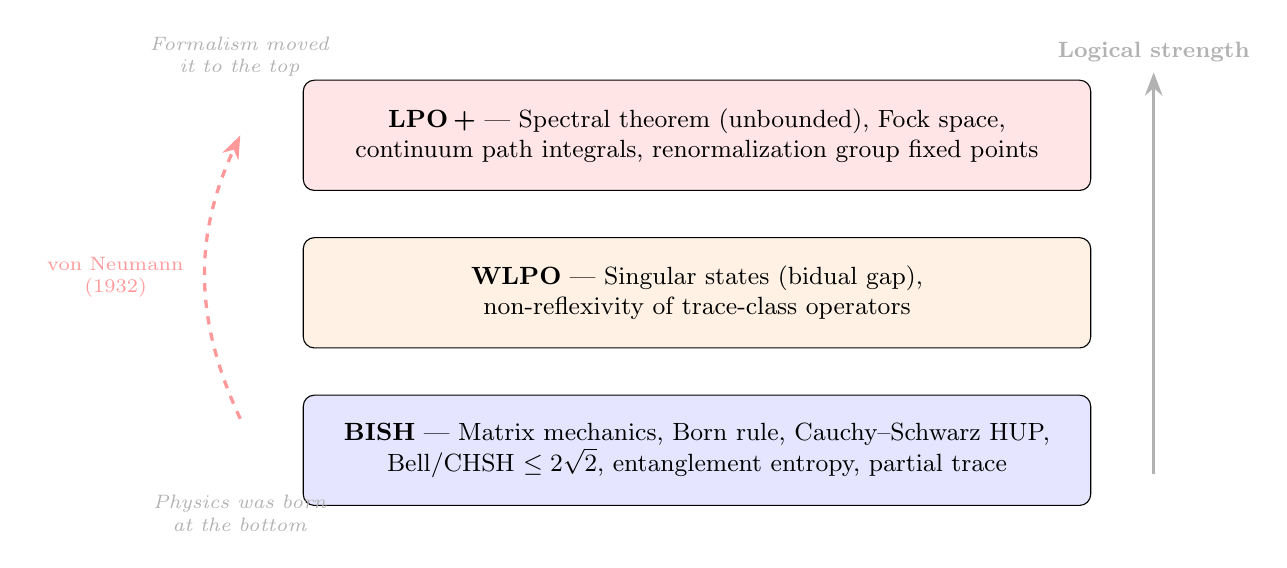
\begin{tikzpicture}[
  >=Stealth,
  every node/.style={font=\small},
  layer/.style={draw, minimum width=10cm, minimum height=1.4cm, align=center, inner sep=4pt}
]
% Bottom layer: BISH
\node[layer, fill=blue!10, rounded corners] (bish) at (0, 0)
  {\textbf{BISH} --- Matrix mechanics, Born rule, Cauchy--Schwarz HUP,\\
   Bell/CHSH $\leq 2\sqrt{2}$, entanglement entropy, partial trace};
% Middle layer: WLPO
\node[layer, fill=orange!10, rounded corners] (wlpo) at (0, 2)
  {\textbf{WLPO} --- Singular states (bidual gap),\\
   non-reflexivity of trace-class operators};
% Top layer: LPO+
\node[layer, fill=red!10, rounded corners] (lpo) at (0, 4)
  {\textbf{LPO\,+} --- Spectral theorem (unbounded), Fock space,\\
   continuum path integrals, renormalization group fixed points};

% Arrow on right
\draw[->, very thick, gray!60] (5.8, -0.3) -- (5.8, 4.8)
  node[above, font=\footnotesize\bfseries, gray!60] {Logical strength};

% Von Neumann arrow
\draw[->, very thick, red!40, dashed] (-5.8, 0.4) to[bend left=25]
  node[left, font=\scriptsize, text width=2cm, align=center] {von Neumann\\(1932)} (-5.8, 4.0);

% Annotation
\node[font=\scriptsize\itshape, gray!60, text width=4cm, align=center] at (-5.8, -0.8)
  {Physics was born\\at the bottom};
\node[font=\scriptsize\itshape, gray!60, text width=4cm, align=center] at (-5.8, 5.0)
  {Formalism moved\\it to the top};

\end{tikzpicture}
\caption{Act~II: the quantum formalization.
Heisenberg's matrix mechanics (1925) is BISH\@.
Von~Neumann's Hilbert space axiomatization (1932) moved the formalism to infinite dimensions.
The empirical content---uncertainty relations, Bell nonlocality, entanglement entropy---remains at BISH\@.
Singular states (WLPO) are mathematical artifacts of the infinite-dimensional framework.}
\label{fig:quantum-layers}
\end{figure}

\begin{keymessage}
Quantum mechanics was born constructive (matrix mechanics = BISH).
Von~Neumann moved it to infinite dimensions (1932).
The HUP, Bell/CHSH, and entanglement entropy are all BISH; singular states cost WLPO\@.
The empirical content stayed at sea level; only the formalism ascended.
\end{keymessage}

% ============================================================
\section{Act~III: The Singularity Detour (1939--1970)}
% ============================================================

In 1939, Einstein published a paper arguing that gravitational collapse could not produce singularities---points of infinite curvature where the equations of general relativity break down \cite{Einstein1939}.
His conviction was principled: ``Every field theory, in our opinion, must therefore adhere to the fundamental principle that singularities of the field are to be excluded.''
Infinite curvature at a point, he reasoned, is not something the physical world produces.
It is a mathematical pathology, an artifact of pushing the formalism past its domain of validity.

The same year, Oppenheimer and Snyder published a paper showing that for a sufficiently massive star, gravitational collapse is inevitable \cite{OppenheimerSnyder1939}.
The community sided with Oppenheimer.
Then, in 1965, Penrose proved the first singularity theorem \cite{Penrose1965}: under generic conditions---trapped surfaces, reasonable energy conditions, global hyperbolicity---spacetime is geodesically incomplete.
Incomplete geodesics are the mathematical signature of singularities.
Hawking extended the result, and the Hawking-Penrose theorems (1970) established singularities as an inescapable feature of general relativity.
Einstein, who died in 1955, was posthumously declared wrong.

Our framework reaches a conclusion that aligns with his, though for entirely different reasons he could not have articulated.
His 1939 argument was physically flawed---it relied on circular orbit stability, which is irrelevant to radial collapse---but his conclusion that singularities are artifacts of the formalism rather than features of the world aligns with the constructive verdict, which locates the artifact precisely at the LPO boundary.

The Penrose singularity theorem has the following logical structure.
The Raychaudhuri equation \cite{Raychaudhuri1955} governs the evolution of the expansion scalar $\theta$ along a geodesic congruence:
\begin{equation}\label{eq:raychaudhuri}
\frac{d\theta}{d\tau} \;=\; -\frac{1}{3}\theta^2 \;-\; \sigma_{\mu\nu}\sigma^{\mu\nu} \;+\; \omega_{\mu\nu}\omega^{\mu\nu} \;-\; R_{\mu\nu}\,u^\mu u^\nu,
\end{equation}
where $\sigma_{\mu\nu}$ is the shear tensor, $\omega_{\mu\nu}$ is the vorticity, $R_{\mu\nu}$ is the Ricci tensor, and $u^\mu$ is the tangent vector.
When the strong energy condition holds ($R_{\mu\nu}u^\mu u^\nu \geq 0$) and vorticity vanishes, the right-hand side is non-positive: the expansion decreases monotonically.
This is a first-order ordinary differential equation on finite parameter intervals---\emph{BISH}.
(The equation displayed is the \emph{timelike} Raychaudhuri equation; Penrose's 1965 theorem uses the \emph{null} version, with $\tfrac{1}{2}\theta^2$ replacing $\tfrac{1}{3}\theta^2$ and vanishing vorticity guaranteed by the twist-free hypothesis on the null geodesic congruence.
The logical structure---finite ODE at BISH, completed limit at LPO---is identical in both cases.)

The non-constructive step comes at the end, and it is the same step as in the thermodynamic limit.
The Penrose theorem asserts a dichotomy on the monotonically decreasing expansion scalar: either the geodesic terminates at finite parameter value (singularity) or it extends forever.
This is Bounded Monotone Convergence---LPO \cite{BridgesVita2006}.
The physical content of the singularity theorem is the Raychaudhuri focusing, which is BISH.
The Kretschmann curvature invariant $K = 48M^2/r^6$ is constructively computable for any $r > 0$, and its divergence is constructively witnessable: for any bound~$B$, one can constructively exhibit~$r_0 > 0$ with $K(r_0) > B$.
This unbounded growth is BISH---not a completed limit.
The completed-limit content resides in the assertion that the geodesic actually \emph{reaches} $r = 0$: that a bounded monotone decreasing sequence of radial coordinates converges to a definite real number.
This is the same bounded monotone convergence equivalence (BMC~$\equiv$~LPO) as in the thermodynamic limit \cite{Lee2026paper13}.
The physics is the focusing; the singularity is where the map says ``here be dragons.''
The territory just keeps going.

Paper~13 \cite{Lee2026paper13} formalizes this decomposition precisely.
The event horizon at $r = 2M$ serves as a \emph{logical boundary}: the exterior geometry (Paper~1) and the interior's finite-time physics---the cycloid geodesic reaching $r = 0$ at proper time $\tau^* = \pi M$, the Kretschmann scalar's constructively witnessable divergence---are BISH.
Only the completed-limit assertion that every bounded monotone trajectory converges to a definite real costs LPO.
The horizon demarcates what can be asserted without surveying an infinite set.

The BMC~$\equiv$~LPO equivalence extends beyond geodesic incompleteness to a fifth physical domain.
Paper~17 \cite{Lee2026paper17} establishes that the Bekenstein-Hawking entropy---$S_{\mathrm{BH}} = A/(4\ell_P^2)$, the entropy assigned to a black hole proportional to its horizon area---is constructively computable for any finite discretization.
But asserting that the entropy per unit area \emph{converges} to the Bekenstein-Hawking value as the discretization is refined costs LPO, through the same bounded monotone convergence mechanism.
Statistical mechanics (Paper~8), general relativity (Paper~13), wave function collapse (Paper~14), Noether's theorem for infinite systems (Paper~15), and now black hole thermodynamics (Paper~17) all pay the same logical price for the same abstract operation: passing from a bounded monotone sequence to its completed limit.
Five domains, one principle.

\textbf{The constructive alternative.}
Einstein was not alone in his discomfort.
Eddington found singularities ``repugnant'' and publicly attacked Chandrasekhar's mass limit calculations in 1935.
The Raychaudhuri equation itself---the constructive core of the singularity theorems---provides all the physical content: quantitative bounds on geodesic convergence over finite parameter intervals.
Every numerical relativity simulation operates at this BISH level, computing finite-precision approximations to geodesic behavior without asserting completed limits---from binary black hole merger simulations to gravitational wave template generation, all finite-precision computations on finite grids.
As recently as 2023, Roy Kerr---discoverer of the Kerr metric for rotating black holes---has argued that physical black holes need not contain singularities \cite{Kerr2023}.
The constructive verdict aligns with a persistent minority view in general relativity: the physics is the focusing, and the singularity is the idealization.

\begin{figure}[ht]
\centering
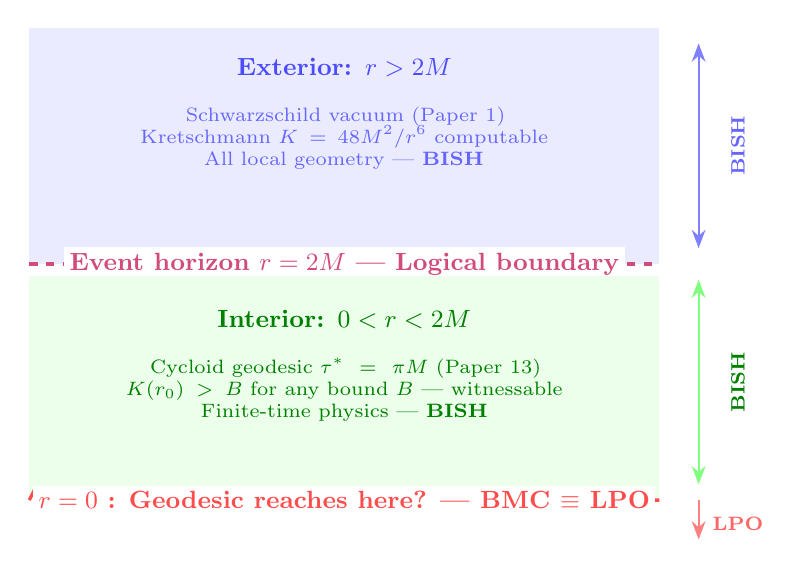
\begin{tikzpicture}[
  >=Stealth,
  every node/.style={font=\small}
]
% Exterior region
\fill[blue!8] (-4, 0) rectangle (4, 3);
\node[font=\small\bfseries, blue!70] at (0, 2.5) {Exterior: $r > 2M$};
\node[font=\scriptsize, blue!60, text width=6cm, align=center] at (0, 1.6)
  {Schwarzschild vacuum (Paper~1)\\Kretschmann $K = 48M^2/r^6$ computable\\All local geometry --- \textbf{BISH}};

% Event horizon
\draw[very thick, dashed, purple!70] (-4, 0) -- (4, 0);
\node[font=\small\bfseries, purple!70, fill=white, inner sep=2pt] at (0, 0) {Event horizon $r = 2M$ --- Logical boundary};

% Interior region
\fill[green!8] (-4, -3) rectangle (4, -0.15);
\node[font=\small\bfseries, green!50!black] at (0, -0.7) {Interior: $0 < r < 2M$};
\node[font=\scriptsize, green!50!black, text width=6.5cm, align=center] at (0, -1.6)
  {Cycloid geodesic $\tau^* = \pi M$ (Paper~13)\\$K(r_0) > B$ for any bound $B$ --- witnessable\\Finite-time physics --- \textbf{BISH}};

% Singularity
\draw[very thick, red!70, decorate, decoration={zigzag, segment length=6pt, amplitude=3pt}]
  (-4, -3) -- (4, -3);
\node[font=\small\bfseries, red!70, fill=white, inner sep=2pt] at (0, -3)
  {$r = 0$ : Geodesic reaches here? --- \textbf{BMC $\equiv$ LPO}};

% Right-side labels
\draw[thick, blue!50, <->] (4.5, 0.2) -- (4.5, 2.8);
\node[font=\scriptsize\bfseries, blue!60, rotate=90] at (5.0, 1.5) {BISH};
\draw[thick, green!50, <->] (4.5, -2.8) -- (4.5, -0.2);
\node[font=\scriptsize\bfseries, green!50!black, rotate=90] at (5.0, -1.5) {BISH};
\draw[thick, red!50, ->] (4.5, -3.0) -- (4.5, -3.5);
\node[font=\scriptsize\bfseries, red!60] at (5.0, -3.3) {LPO};

\end{tikzpicture}
\caption{Act~III: the event horizon as a logical boundary.
The exterior geometry and the interior's finite-time physics are both BISH\@.
The singularity---the assertion that a bounded monotone trajectory converges to a definite real---costs LPO\@.
The horizon demarcates what can be asserted without surveying an infinite set (Paper~13).}
\label{fig:blackhole}
\end{figure}

\begin{keymessage}
The Raychaudhuri focusing equation is BISH\@.
The Kretschmann divergence is constructively witnessable.
Only the assertion ``the geodesic reaches $r = 0$'' costs LPO---the same BMC equivalence as the thermodynamic limit.
The event horizon is a logical boundary (Paper~13).
\end{keymessage}

% ============================================================
\section{Act~IV: The Greatest Predictions from the Smallest Logic (1947--1975)}
% ============================================================

Between 1947 and 1975, quantum field theory delivered the cellar-and-cathedral pattern of Section~1 at industrial scale.
Every Feynman diagram computation---the actual source of QFT's legendary precision---is BISH: finite integrals, finite arithmetic, controlled error.
But the formalism grew a new cathedral above the cellar.
Fock space completeness, renormalization group fixed points, and the vacuum state all live at LPO or beyond.
And the path integral---a formal ``integral'' over an infinite-dimensional configuration space for which no rigorous measure exists---requires choice principles far stronger still.

Yet the predictions are spectacular.
The formalism works---not because the infinite-dimensional apparatus is physically real, but because it is an effective mnemonic for organizing BISH-level computations.
The path integral is a beautiful legend on the map explaining how to read the contour lines.
The contour lines---the Feynman diagrams---are the actual geography.

The Yang-Mills mass gap problem---one of the seven Clay Millennium Prize Problems---asks for a proof that a quantum field theory satisfying certain axioms has a positive mass gap.
The axioms involve infinite-dimensional structures (Wightman axioms, Osterwalder-Schrader axioms) that are LPO or stronger.
If the empirical content of Yang-Mills theory is BISH---and lattice QCD already computes hadron masses from first principles at BISH---the Millennium Problem asks for a rigorous construction of Yang-Mills in the \emph{continuum limit}, connecting the BISH-level lattice computation to the LPO-level continuum formalism.
It is a question about the \emph{map}: whether the infinite-dimensional formalization faithfully represents the finite-dimensional physics.
The physical predictions do not depend on the answer.

Not every non-constructive scaffold is idle, however---some are idle and \emph{known} to be idle.
Paper~18 \cite{Lee2026paper18} establishes a \emph{Scaffolding Principle}: the Standard Model's Yukawa renormalization group evolution---the machinery that runs fermion masses from high to low energies---is entirely constructive (BISH).
Removing the non-constructive scaffolding from the fermion mass problem reveals nothing new: the hierarchy problem persists at BISH, and the scaffolding, though idle, does not obstruct the physics.
This is a negative result that matters.
It means the mass hierarchy is not an artifact of classical logic; it is a genuine structural feature of the Standard Model that survives constructivization intact.
The cellar-and-cathedral pattern applies, but in reverse: the cathedral was not hiding anything from the cellar.

\textbf{The constructive alternative.}
The fragility of the formalism was recognized from within.
Dyson showed in 1952 \cite{Dyson1952} that the perturbation series in QED \emph{diverges}---it is asymptotic, not convergent.
The perturbation series is asymptotic, not convergent---a mathematical property of the \emph{approximation scheme}, not of the physical theory itself.
Non-perturbative methods (lattice QCD, resummation techniques) access the theory without relying on convergence of the perturbation series.
All twelve decimal places of the $g{-}2$ prediction come from truncating the perturbation series at finite order---BISH operations that are independent of whether the full series converges.
Haag's theorem (1955) \cite{Haag1996} demonstrated that the Fock space representation for free fields is unitarily inequivalent to the representation for interacting fields---the infinity of inequivalent representations is an artifact of infinite-dimensional Hilbert spaces.
In finite dimensions, the Stone-von~Neumann theorem guarantees a unique representation; the problem arises exclusively from the passage to infinite dimension.
The Glimm-Jaffe constructive quantum field theory program (1968--1981) \cite{GlimmJaffe1981} attempted to build QFT on rigorous mathematical foundations and succeeded in two and three spacetime dimensions---but the physically relevant four-dimensional case remains open, which is essentially the content of the Millennium Prize.
Every actual confirmed prediction of QFT---lattice QCD calculations of hadron masses, QED computations of magnetic moments---is a computation on a finite lattice or at finite loop order.
The constructive alternative is what physicists already do.

\begin{figure}[ht]
\centering
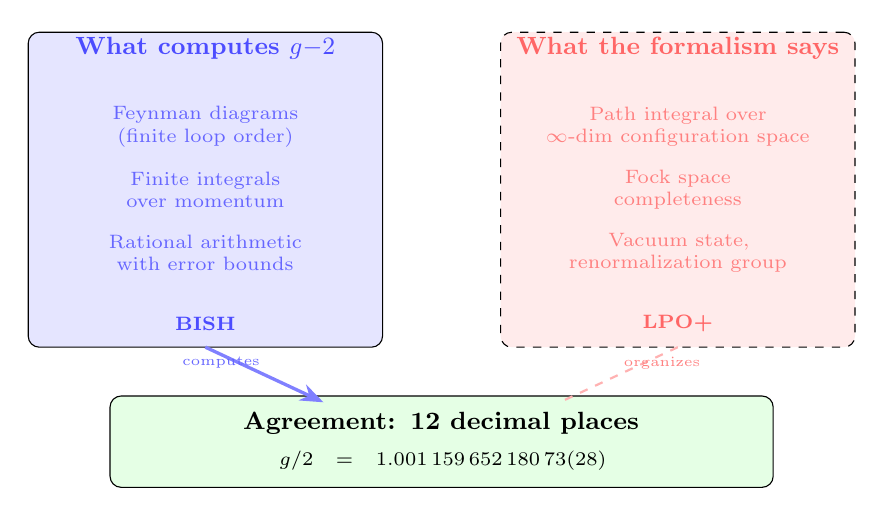
\begin{tikzpicture}[
  >=Stealth,
  every node/.style={font=\small},
  col/.style={draw, rounded corners, minimum width=4.5cm, align=center, inner sep=6pt}
]
% Left column: what actually computes
\node[col, fill=blue!10, minimum height=4cm] (cellar) at (-3, 2) {};
\node[font=\small\bfseries, blue!70] at (-3, 3.8) {What computes $g{-}2$};
\node[font=\scriptsize, blue!60, text width=3.8cm, align=center] at (-3, 2.8)
  {Feynman diagrams\\(finite loop order)};
\node[font=\scriptsize, blue!60, text width=3.8cm, align=center] at (-3, 2.0)
  {Finite integrals\\over momentum};
\node[font=\scriptsize, blue!60, text width=3.8cm, align=center] at (-3, 1.2)
  {Rational arithmetic\\with error bounds};
\node[font=\scriptsize\bfseries, blue!70] at (-3, 0.3) {BISH};

% Right column: the formalism
\node[col, fill=red!8, minimum height=4cm, dashed] (cath) at (3, 2) {};
\node[font=\small\bfseries, red!60] at (3, 3.8) {What the formalism says};
\node[font=\scriptsize, red!50, text width=3.8cm, align=center] at (3, 2.8)
  {Path integral over\\$\infty$-dim configuration space};
\node[font=\scriptsize, red!50, text width=3.8cm, align=center] at (3, 2.0)
  {Fock space\\completeness};
\node[font=\scriptsize, red!50, text width=3.8cm, align=center] at (3, 1.2)
  {Vacuum state,\\renormalization group};
\node[font=\scriptsize\bfseries, red!60] at (3, 0.3) {LPO+};

% Result
\node[draw, rounded corners, fill=green!10, font=\small\bfseries, text width=8cm, align=center, inner sep=6pt]
  (result) at (0, -1.2) {Agreement: 12 decimal places\\[2pt]
  \normalfont\scriptsize $g/2 = 1.001\,159\,652\,180\,73(28)$};

% Arrow from cellar to result
\draw[->, very thick, blue!50] (-3, 0) -- (-1.5, -0.7);
% Disconnected from cathedral
\draw[thick, red!30, dashed] (3, 0) -- (1.5, -0.7);
\node[font=\tiny, red!50] at (2.8, -0.2) {organizes};
\node[font=\tiny, blue!60] at (-2.8, -0.2) {computes};

\end{tikzpicture}
\caption{Act~IV: the most precise prediction in physics.
The $g{-}2$ computation uses finite Feynman diagrams (BISH, solid arrow).
The infinite-dimensional formalism (LPO+, dashed) organizes the computation
but does not contribute to the numerical result.
Twelve decimal places of agreement come from the cellar, not the cathedral.}
\label{fig:g-minus-2}
\end{figure}

% ============================================================
\section{Act~V: The Interpretive Crisis (1975--Present)}
% ============================================================

After the Standard Model was completed in the mid-1970s, the data stream slowed.
The model agreed with every experiment.
New phenomena required higher energies, bigger accelerators, longer timescales, and more money.
Theorists, no longer constrained by a steady flow of surprises from the laboratory, began exploring the mathematical formalism itself.

What they explored was the non-constructive superstructure.

String theory posits a landscape of $10^{500}$ vacuum states---solutions to the equations of the theory that represent possible universes.
This is an assertion about the structure of an infinite-dimensional space of solutions.
No finite experiment can probe it.
The many-worlds interpretation of quantum mechanics takes the universal wave function literally, asserting the real physical existence of a branching structure in infinite-dimensional Hilbert space.
No measurement can access the other branches.
The black hole information paradox asks what happens to quantum information at a singularity---combining two LPO-level idealizations (the singularity and the infinite-dimensional state space) into a single problem.

From the perspective of the constructive hierarchy, these debates share a structural feature: they are about properties of mathematical objects that live at LPO or higher.
They are questions about the formalism, not about the world.
If you accept that the empirical content of physics is BISH, then a question that can only be \emph{formulated} using LPO or LEM is a question about the mathematical map, not the physical territory.

This diagnosis of the stagnation of theoretical physics is different from, and sharper than, existing critiques.
It does not blame aesthetics, as Hossenfelder does in \emph{Lost in Math}.
It does not blame unfalsifiability, as Woit does in \emph{Not Even Wrong}.
It does not blame sociology, as Smolin does in \emph{The Trouble with Physics}.
It identifies a \emph{structural} correlate: the programmes that have failed to produce testable predictions operate at logical levels that are inherently disconnected from empirical content.
You can explore those levels forever and never produce a prediction that a finite laboratory can test, because the logical distance between the formalism and the predictions is too large.
The formalism is not wrong; it is \emph{idle}---machinery not connected to any output.

A qualification is essential.
Not all post-1975 theoretical work explores the non-constructive superstructure.
Lattice QCD (building on Wilson's 1974 construction \cite{Wilson1974}) has matured into a BISH-level computational programme that predicts hadron masses to percent-level accuracy.
Effective field theory (Weinberg, 1979 onward) organizes finite-order calculations systematically without claiming convergence of the full perturbation series.
Tensor network methods (White 1992, Vidal 2003 onward) provide finite-dimensional variational approaches to quantum many-body systems that avoid infinite-dimensional Hilbert spaces entirely.
Validated numerics and computer-assisted proofs employ interval arithmetic at BISH.
The diagnosis targets specifically those programmes---the string landscape, the multiverse, the information paradox---that operate at logical levels inherently disconnected from finite experiment.
The idle machinery is not ``all post-1975 theory'' but the subset that explores the non-constructive superstructure without producing BISH-level predictions.

\begin{figure}[ht]
\centering
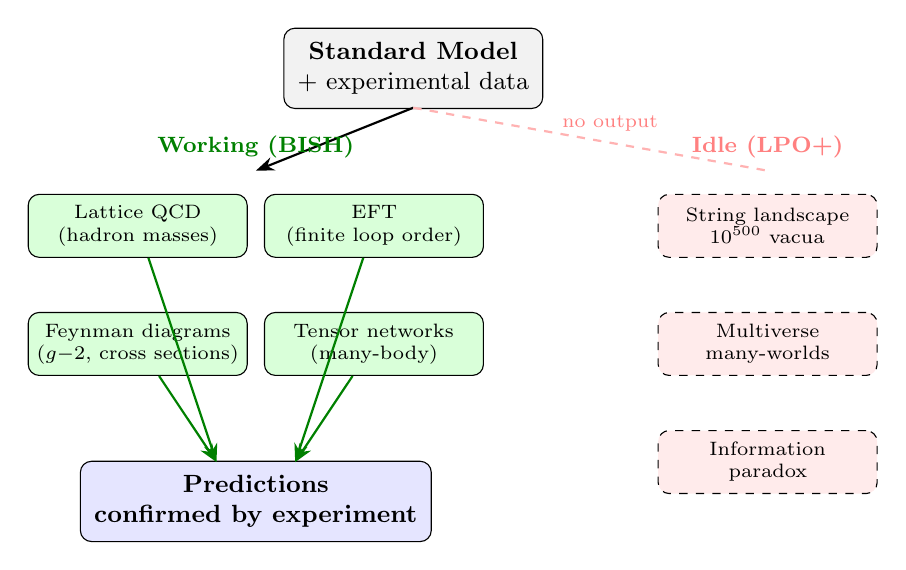
\begin{tikzpicture}[
  >=Stealth,
  every node/.style={font=\small},
  gear/.style={draw, rounded corners, minimum height=0.8cm, align=center, inner sep=4pt, font=\scriptsize}
]
% Input
\node[draw, rounded corners, fill=gray!10, minimum width=3cm, align=center, inner sep=5pt]
  (input) at (0, 3.5) {\textbf{Standard Model}\\+ experimental data};

% Working machinery (BISH)
\node[gear, fill=green!15, text width=2.5cm] (lqcd) at (-3.5, 1.5) {Lattice QCD\\(hadron masses)};
\node[gear, fill=green!15, text width=2.5cm] (eft) at (-0.5, 1.5) {EFT\\(finite loop order)};
\node[gear, fill=green!15, text width=2.5cm] (feyn) at (-3.5, 0) {Feynman diagrams\\($g{-}2$, cross sections)};
\node[gear, fill=green!15, text width=2.5cm] (tensor) at (-0.5, 0) {Tensor networks\\(many-body)};

% Idle machinery (LPO+)
\node[gear, fill=red!8, dashed, text width=2.5cm] (string) at (4.5, 1.5) {String landscape\\$10^{500}$ vacua};
\node[gear, fill=red!8, dashed, text width=2.5cm] (multi) at (4.5, 0) {Multiverse\\many-worlds};
\node[gear, fill=red!8, dashed, text width=2.5cm] (info) at (4.5, -1.5) {Information\\paradox};

% Output
\node[draw, rounded corners, fill=blue!10, minimum width=3cm, align=center, inner sep=5pt, font=\small\bfseries]
  (output) at (-2, -2) {Predictions\\confirmed by experiment};

% Arrows
\draw[->, thick] (0, 3.0) -- (-2, 2.2);
\draw[->, thick, green!50!black] (lqcd) -- (-2.5, -1.5);
\draw[->, thick, green!50!black] (eft) -- (-1.5, -1.5);
\draw[->, thick, green!50!black] (feyn) -- (-2.5, -1.5);
\draw[->, thick, green!50!black] (tensor) -- (-1.5, -1.5);

% No connection from idle
\draw[thick, red!30, dashed] (0, 3.0) -- (4.5, 2.2);
\node[font=\scriptsize, red!50] at (2.5, 2.8) {no output};

% Labels
\node[font=\footnotesize\bfseries, green!50!black] at (-2, 2.5) {Working (BISH)};
\node[font=\footnotesize\bfseries, red!50] at (4.5, 2.5) {Idle (LPO+)};

\end{tikzpicture}
\caption{Act~V: working machinery vs.\ idle machinery.
Post-1975 physics divides into programmes that produce BISH-level predictions confirmed by experiment
(left, green) and programmes that explore the non-constructive superstructure without
empirical output (right, red/dashed).
The diagnosis is structural: the idle machinery operates at logical levels disconnected from finite experiment.}
\label{fig:idle-machinery}
\end{figure}

The constructive hierarchy suggests a diagnosis and a remedy: the next breakthrough may require \emph{less} logical structure, not more---the identification of which parts of the existing formalism are physically idle and their careful removal.

\textbf{The constructive alternative.}
Bishop's \emph{Foundations of Constructive Analysis} (1967) \cite{Bishop1967} proved that the core of mathematical analysis survives constructively; his 1973 lectures diagnosed contemporary mathematics as suffering from a ``schizophrenia'' between formal manipulation and computational meaning.
Since 2019, Nicolas Gisin---a physicist with Nobel-adjacent credentials in quantum nonlocality---has argued that real numbers are ``the hidden variables of classical physics,'' that intuitionistic mathematics is the natural language for finite physical systems, and that the apparent determinism of classical mechanics is an artifact of using real numbers with infinite information content \cite{Gisin2020, Gisin2021}.
Gisin provides the philosophical vision; our programme supplies the formal precision his broad-brush argument lacks (see Section~\ref{sec:thesis}).

\begin{keymessage}
Post-Standard-Model theoretical physics explores logical levels disconnected from experiment.
The diagnosis is structural: formalism at LPO+ cannot produce BISH-level predictions.
Working programmes (lattice QCD, EFT, tensor networks) remain at BISH\@.
The idle machinery is not all post-1975 theory---only the subset that explores the non-constructive superstructure.
\end{keymessage}


% ============================================================
\section{The Logical Geography: What the Proofs Show}
% ============================================================

The preceding narrative rests on a specific body of evidence: a calibration table mapping layers of mathematical physics to their precise position in the constructive hierarchy.
Each entry is machine-verified in the Lean~4 proof assistant, using either constructive reverse mathematics (CRM) over the Mathlib library \cite{Ishihara2006, BridgesVita2006} or an axiom-calibration framework in standalone Lean.

\begin{figure}[ht]
\centering
\resizebox{0.92\textwidth}{!}{%
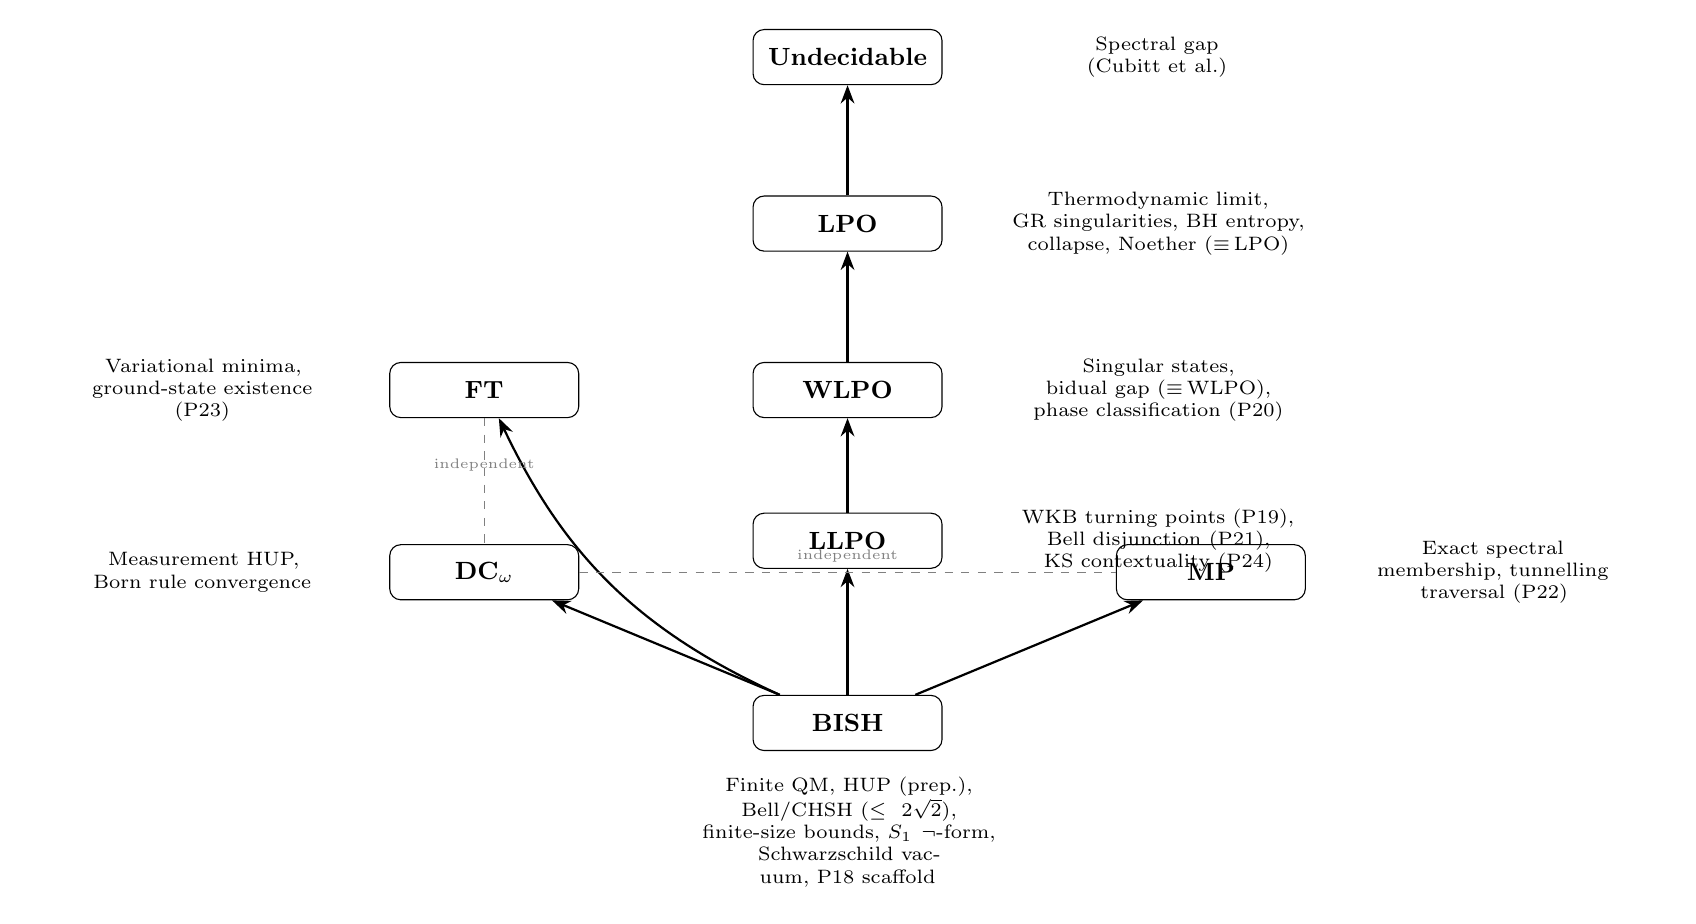
\begin{tikzpicture}[
  node distance=1.4cm and 2.8cm,
  principle/.style={draw, rounded corners, minimum width=2.4cm, minimum height=0.7cm, font=\small\bfseries},
  physlabel/.style={font=\scriptsize, text width=4.2cm, align=center},
  >=Stealth
]
% Main spine
\node[principle] (bish) {BISH};
\node[principle, above=1.6cm of bish] (llpo) {LLPO};
\node[principle, above=1.2cm of llpo] (wlpo) {WLPO};
\node[principle, above=of wlpo] (lpo) {LPO};
\node[principle, above=of lpo] (undec) {Undecidable};

% Orthogonal branches
\node[principle, above left=1.2cm and 2.2cm of bish] (dc) {DC$_\omega$};
\node[principle, above right=1.2cm and 2.2cm of bish] (mp) {MP};
\node[principle, left=2.2cm of wlpo] (ft) {FT};

% Edges (Hasse diagram: only covering relations)
\draw[thick, ->] (bish) -- (dc);
\draw[thick, ->] (bish) -- (mp);
\draw[thick, ->] (bish) -- (llpo);
\draw[thick, ->] (llpo) -- (wlpo);
\draw[thick, ->] (wlpo) -- (lpo);
\draw[thick, ->] (lpo) -- (undec);
\draw[thick, ->] (bish) to[bend left=20] (ft);

% Physical labels
\node[physlabel, below=0.2cm of bish] {Finite QM, HUP (prep.),\\Bell/CHSH ($\leq 2\sqrt{2}$),\\finite-size bounds, $S_1\;\neg$-form,\\Schwarzschild vacuum, P18 scaffold};
\node[physlabel, left=0.15cm of dc] {Measurement HUP,\\Born rule convergence};
\node[physlabel, right=0.15cm of mp] {Exact spectral\\membership, tunnelling\\traversal (P22)};
\node[physlabel, left=0.15cm of ft] {Variational minima,\\ground-state existence\\(P23)};
\node[physlabel, right=0.5cm of llpo] {WKB turning points (P19),\\Bell disjunction (P21),\\KS contextuality (P24)};
\node[physlabel, right=0.5cm of wlpo] {Singular states,\\bidual gap ($\equiv$\,WLPO),\\phase classification (P20)};
\node[physlabel, right=0.5cm of lpo] {Thermodynamic limit,\\GR singularities, BH entropy,\\collapse, Noether ($\equiv$\,LPO)};
\node[physlabel, right=0.5cm of undec] {Spectral gap\\(Cubitt et al.)};

% Orthogonality annotations
\draw[dashed, gray] (dc) -- node[above, font=\tiny, gray] {independent} (mp);
\draw[dashed, gray] (ft) -- node[above, font=\tiny, gray] {independent} (dc);

\end{tikzpicture}%
}% end resizebox
\caption{The logical geography of mathematical physics: a Hasse diagram (v3.0).
Arrows indicate strict implication over BISH\@. The omniscience spine
(BISH $<$ LLPO $<$ WLPO $<$ LPO) forms the dominant vertical chain. DC$_\omega$, MP, and FT
occupy orthogonal positions: none implies any other, and none implies WLPO.
Physical layers are annotated with their calibrated logical cost from Papers~2--24.
All entries are machine-verified; ``$\equiv$'' denotes proven equivalence over BISH.}
\label{fig:hasse}
\end{figure}

The calibration table is displayed in Figure~\ref{fig:hasse}.
Return to the mountain metaphor.

\textbf{Sea level (BISH).}
Everything a laboratory does lives here.
Finite quantum mechanics: unitary evolution, Born rule probabilities, measurements on finite-dimensional systems.
Preparation uncertainty: the Robertson-Schr\"odinger inequality~\eqref{eq:rs-inequality}, a pure Cauchy-Schwarz argument.
Bell nonlocality: the Tsirelson bound~\eqref{eq:chsh} on CHSH correlations.
Entanglement entropy of qubit systems: the Bell singlet partial trace yields $\operatorname{Tr}_B(|\Psi^-\rangle\langle\Psi^-|) = \tfrac{1}{2}I_2$, giving maximal entanglement entropy $h(1/2) = \log 2$---all explicit matrix arithmetic, BISH.
Finite-size error bounds~\eqref{eq:ising-bound} for the one-dimensional Ising model.
Local general relativity: the Raychaudhuri focusing equation~\eqref{eq:raychaudhuri}, the Schwarzschild vacuum solution with its constructively computable Kretschmann invariant $K = 48M^2/r^6$.
All of these are provable without any omniscience principle or appeal to the law of excluded middle.

\textbf{The foothills (Dependent Choice, Markov's Principle, Fan Theorem).}
Measurement uncertainty---extracting classical statistics from an infinite sequence of quantum measurements---requires Dependent Choice \cite{Lee2026g}.
The measurement problem itself (Paper~16 \cite{Lee2026paper16}) is a DC$_\omega$ phenomenon: the controversy over wave function collapse reduces to a disagreement about whether to accept dependent countable choice for the convergence of relative frequencies.
Exact spectral membership---asserting that a specific value belongs to the spectrum of an operator---requires Markov's Principle \cite{Lee2026f}.
The tunnelling traversal time controversy (Paper~22 \cite{Lee2026paper22}) turns on MP: inferring that an unstable nucleus will eventually decay because it cannot persist forever is exactly the Markov inference.
The Fan Theorem occupies a third independent foothill: asserting that a continuous function on a compact set attains its minimum---a staple of variational principles, ground-state existence arguments, and equilibrium optimization---requires FT \cite{Lee2026paper23}, which is independent of the entire omniscience spine.
These three principles are independent of each other and independent of WLPO.
The logical geography is not a simple linear chain; it has lateral dimensions.

\textbf{The LLPO ledge.}
Between the foothills and the mountainside lies LLPO---the principle that determines the sign of a nonzero real.
The WKB approximation has three logical tiers: the tunnelling probability through a specific barrier is BISH, but asserting that a general continuous potential has classical turning points costs LLPO \cite{Lee2026paper19}.
Bell's disjunction---``either locality fails or realism fails''---costs LLPO \cite{Lee2026paper21}.
Kochen-Specker contextuality has exactly the same logical cost \cite{Lee2026paper24}: two physically unrelated impossibility theorems are the same logical phenomenon.

\textbf{The mountainside (WLPO).}
Singular states---functionals in the bidual of the trace-class operators that correspond to no density matrix---require WLPO to construct \cite{Lee2026a, Lee2026b}.
The bidual gap, the separation between physical states and mathematical artifacts of the infinite-dimensional formalism, costs exactly WLPO.
Phase classification of the 1D Ising model---asking ``is the magnetization zero or not?''---also costs WLPO \cite{Lee2026paper20}: the logical price depends on the question, not just the system.

\textbf{The summit (LPO).}
The thermodynamic limit: the assertion that the free energy per particle converges to a definite real number as the system size grows without bound.
This is equivalent to LPO over constructive mathematics---proved for the one-dimensional Ising model \cite{Lee2026c} and verified across two independent mathematical formulations (transfer-matrix and combinatorial \cite{Lee2026e}), establishing that the logical cost is intrinsic to the physics, not an artifact of the proof technique.
The same BMC~$\equiv$~LPO equivalence governs geodesic incompleteness in general relativity \cite{Lee2026paper13}, wave function collapse as the infinite-time limit of decoherence \cite{Lee2026paper14}, global energy conservation for infinite systems via Noether's theorem \cite{Lee2026paper15}, and Bekenstein-Hawking entropy convergence \cite{Lee2026paper17}.
This \emph{domain invariance}---the same logical cost appearing in five independent physical domains through the same abstract principle---strengthens the evidence that the costs are intrinsic to the operation of passing from a bounded monotone sequence to its limit, regardless of the physical domain that produces the sequence.

\textbf{Beyond the summit (undecidable).}
The spectral gap problem---whether the Hamiltonian of an infinite lattice system has a gap above the ground state energy---is undecidable in the sense of Turing: no algorithm can determine the answer from the Hamiltonian's local interaction rules \cite{Cubitt2015}.
This is not ``a level above LEM'' in the logical hierarchy; it is an orthogonal phenomenon.
LEM does not help you compute an uncomputable function.
Undecidability means that the idealization strategy hits a different kind of ceiling---not insufficient logical strength, but the inherent limitation of algorithmic procedures applied to infinite lattice systems.
The summit of the omniscience hierarchy (LPO) and Turing undecidability are distinct obstructions, and conflating them would misrepresent both.

Yet the two hierarchies share a common boundary.
For any \emph{finite} lattice, the spectral gap is a computable real number---eigenvalues of a finite Hermitian matrix are BISH, and the question ``is the gap above~$\varepsilon$?'' is decidable by rational approximation.
The undecidability of Cubitt et~al.\ enters only through the thermodynamic limit $N \to \infty$---the same limit that costs LPO in the Ising calibration.
The constructive hierarchy and the computability hierarchy are orthogonal axes, but they agree on where the physics--formalism boundary falls: finite systems sit at BISH/decidable, and infinite idealizations sit above BISH in both.
A similar pattern appears in the foundations of quantum correlations.
The set of correlations achievable by finite-dimensional quantum systems is identical whether formalized via tensor products or commuting operators, and the Tsirelson bound $2\sqrt{2}$ holds in both formalizations at BISH \cite{Lee2026paper11}.
Ji, Natarajan, Vidick, Wright, and Yuen showed that this equivalence fails catastrophically in infinite dimensions: the membership problem for infinite-dimensional commuting-operator correlations is RE-complete---as hard as the halting problem \cite{JNVWY2021}.
The physical correlations, preparable with finite entanglement and measurable by finite apparatus, are BISH and formalization-invariant.
The mathematical excess---correlations requiring infinite entanglement in infinite-dimensional spaces---is where the formalizations diverge, and the divergence reaches the highest levels of the computability hierarchy.
Neither result has been calibrated against the omniscience hierarchy (that would require proving specific equivalences with WLPO, LPO, or higher principles, which remains open), but both confirm the programme's central pattern: physical content at BISH, with logical cost increasing monotonically as the formalism extends beyond the finite.

Two features of this table deserve emphasis.

First, \emph{formulation-invariance}.
The LPO cost of the thermodynamic limit was derived independently via two completely different mathematical routes: a transfer-matrix method using eigenvalue analysis and linear algebra, and a purely combinatorial method using bond variables and a binomial parity sieve with no matrices or functional analysis \cite{Lee2026e}.
The axiom profiles are identical.
This is evidence that the logical cost is a property of the physics, not of the mathematician's choice of formalism.

Second, \emph{machine verification}.
These results are not informal arguments about what ``should'' be constructive.
They are Lean~4 proof terms, machine-checked end-to-end, with \texttt{\#print axioms} certificates that list every non-constructive axiom used in each proof.
The total is approximately 18,500~lines of formally verified code.
The proof assistant enforces the logical bookkeeping that human mathematicians cannot reliably perform: it ensures that no classical axiom sneaks in through a library import, a typeclass resolution, or an unnoticed appeal to decidability.

\begin{keymessage}
The calibration table maps physics to exact logical levels, machine-verified in ${\sim}18{,}500$ lines of Lean~4.
Key findings: \emph{formulation-invariance} (same cost via different proofs), \emph{domain invariance} (same cost in five physical domains), and \emph{observable-dependent cost} (same system, different question $\Rightarrow$ different level) show the logical costs are intrinsic, not artifacts of the formalism.
\end{keymessage}

% ============================================================
\section{What Could Have Been Done Instead}
% ============================================================

The calibration table is not merely a diagnosis; it suggests a therapy.
The remarkable fact is that physicists \emph{already compute at BISH}---they just don't know it.
The constructive alternatives to the classical formalism are not radical proposals for a new physics.
They are descriptions of what physicists actually do: finite-size error bounds instead of the thermodynamic limit~\eqref{eq:ising-bound}, the Cauchy-Schwarz inequality instead of spectral theory for uncertainty~\eqref{eq:rs-inequality}, finite-dimensional linear algebra for Bell nonlocality~\eqref{eq:chsh}, finite-parameter differential equations for gravitational focusing~\eqref{eq:raychaudhuri}, and finite-order Feynman diagrams instead of path integrals.
In every case the constructive alternative is what the working physicist is already doing.
The formalism merely pretends otherwise.

Moreover, several post-war developments in mathematical physics are themselves constructive frameworks, often unrecognized as such:
\begin{itemize}[nosep]
\item \textbf{Wilson's lattice gauge theory (1974) \cite{Wilson1974}}: a rigorous,
  finite-dimensional framework for non-perturbative QFT\@. Lattice QCD computes
  hadron masses, the proton charge radius, and quark masses from first
  principles---all on finite grids with controlled errors. This is BISH\@.
\item \textbf{Effective field theory} (Weinberg, 1979+): a systematic
  organizing principle that keeps calculations at finite loop order without
  claiming convergence of the full perturbation series.
\item \textbf{Tensor network methods} (White 1992, Vidal 2003+):
  finite-dimensional variational approaches to quantum many-body systems
  (DMRG, MERA, PEPS) that avoid infinite-dimensional Hilbert spaces entirely.
\item \textbf{Validated numerics}: interval arithmetic and computer-assisted
  proofs that produce rigorous finite-precision bounds---constructive
  mathematics in practice.
\item \textbf{Constructive quantum foundations} (this programme, 2026):
  the constructive calibration of Bell nonlocality (BISH), the measurement
  problem (DC$_\omega$), tunnelling traversal (MP), WKB turning points (LLPO),
  and variational principles (FT) provides a complete logical anatomy of
  quantum mechanics that separates physical content from formalism at
  every level of the hierarchy.
\end{itemize}
The constructive alternative is not a hypothetical programme; it is how much of contemporary computational physics already operates.

\begin{figure}[ht]
\centering
\resizebox{\textwidth}{!}{%
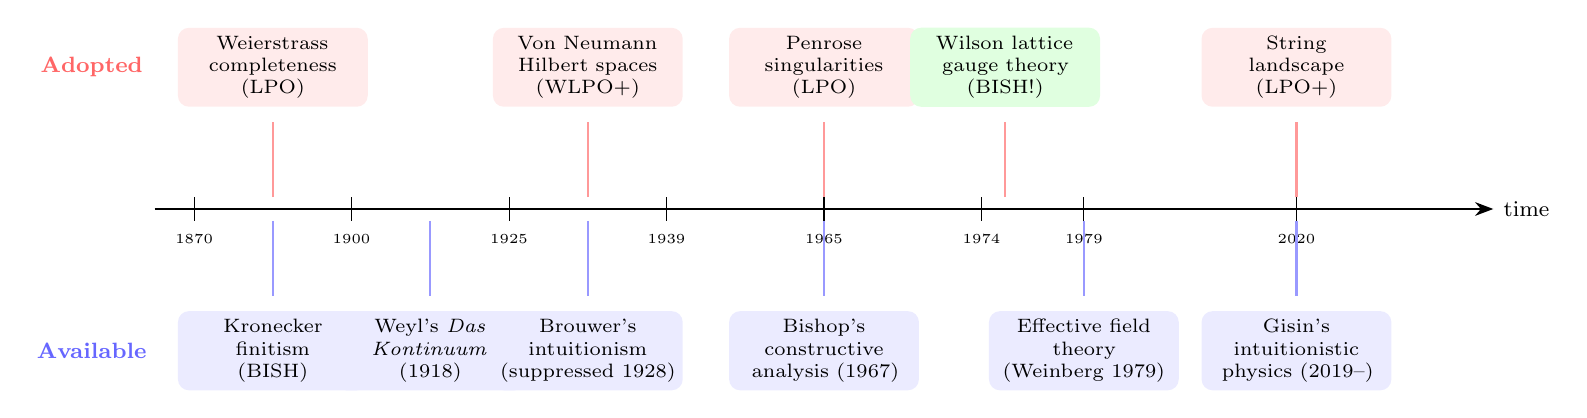
\begin{tikzpicture}[
  >=Stealth,
  every node/.style={font=\scriptsize},
  event/.style={circle, fill, inner sep=1.5pt},
  adopted/.style={font=\scriptsize, text width=2.2cm, align=center, fill=red!8, rounded corners, inner sep=3pt},
  alternative/.style={font=\scriptsize, text width=2.2cm, align=center, fill=blue!8, rounded corners, inner sep=3pt}
]
% Timeline
\draw[thick, ->] (0,0) -- (17, 0) node[right] {\footnotesize time};
% Tick marks
\foreach \x/\y in {0.5/1870, 2.5/1900, 4.5/1925, 6.5/1939, 8.5/1965, 10.5/1974, 11.8/1979, 14.5/2020} {
  \draw (\x, -0.15) -- (\x, 0.15);
  \node[below, font=\tiny] at (\x, -0.2) {\y};
}
% Upper track: what was adopted (red-tinted)
\node[adopted] at (1.5, 1.8) {Weierstrass\\completeness\\(LPO)};
\node[adopted] at (5.5, 1.8) {Von Neumann\\Hilbert spaces\\(WLPO+)};
\node[adopted] at (8.5, 1.8) {Penrose\\singularities\\(LPO)};
\node[adopted, fill=green!12] at (10.8, 1.8) {Wilson lattice\\gauge theory\\(BISH!)};
\node[adopted] at (14.5, 1.8) {String\\landscape\\(LPO+)};
% Lower track: what was available (blue-tinted)
\node[alternative] at (1.5, -1.8) {Kronecker\\finitism\\(BISH)};
\node[alternative] at (3.5, -1.8) {Weyl's \emph{Das\\Kontinuum}\\(1918)};
\node[alternative] at (5.5, -1.8) {Brouwer's\\intuitionism\\(suppressed 1928)};
\node[alternative] at (8.5, -1.8) {Bishop's\\constructive\\analysis (1967)};
\node[alternative] at (11.8, -1.8) {Effective field\\theory\\(Weinberg 1979)};
\node[alternative] at (14.5, -1.8) {Gisin's\\intuitionistic\\physics (2019--)};
% Arrows connecting to timeline
\foreach \x in {1.5, 5.5, 8.5, 10.8, 14.5} {
  \draw[red!40, thick] (\x, 0.15) -- (\x, 1.1);
}
\foreach \x in {1.5, 3.5, 5.5, 8.5, 11.8, 14.5} {
  \draw[blue!40, thick] (\x, -0.15) -- (\x, -1.1);
}
% Labels for tracks
\node[font=\footnotesize\bfseries, red!60] at (-0.8, 1.8) {Adopted};
\node[font=\footnotesize\bfseries, blue!60] at (-0.8, -1.8) {Available};
\end{tikzpicture}%
}% end resizebox
\caption{The road not taken. At every stage where classical logic was imported into
physics (upper track, red), a constructive alternative was available (lower track, blue).
Wilson's lattice gauge theory (green, 1974) is the exception: an adopted framework
that is itself BISH\@.
The constructive road was not taken---not because it was mathematically inadequate,
but because the classical road was more convenient and its logical cost was invisible.}
\label{fig:timeline}
\end{figure}

\begin{keymessage}
At every stage, constructive alternatives existed (Figure~\ref{fig:timeline}).
Lattice QCD, effective field theory, tensor networks, and validated numerics are already BISH frameworks.
The constructive alternative is not a hypothetical programme---it is what physicists already do.
\end{keymessage}

\bigskip

\textbf{The programme's trajectory.} Before stating the thesis, it is worth pausing to trace how the programme's understanding evolved. The full intellectual history is given in Paper~10, \S6; here we sketch the arc in broad strokes. Looking back, the programme passed through four phases, each prompted by the results and limitations of the phase before it.

\emph{Phase~1: First probes} (Papers~2, 4, 6, 7). The earliest papers asked whether constructive questions about physics had non-trivial answers. They did: specific principles --- WLPO for the bidual gap, DC$_\omega$ for measurement uncertainty, MP for exact spectral membership --- attached to specific pieces of physics. But the approach was unsystematic. Most results were one-directional (``this theorem \emph{requires} at least WLPO'') rather than tight equivalences. The question had been shown to be interesting; the technique for answering it precisely was still missing.

\emph{Phase~2: The BISH-LPO paradigm} (Papers~8, 9, 11, 13, 14, 15). Paper~8's discovery that the thermodynamic limit of the 1D Ising model is \emph{equivalent} to LPO (via BMC) gave the programme its paradigm: finite physics is BISH, completed limits cost LPO, and the equivalence is tight in both directions. Papers~9, 11, 13, 14, and~15 confirmed this across five domains --- statistical mechanics, quantum information, general relativity, decoherence, and conservation laws --- and established that the cost is formulation-invariant. The pattern was unmistakable.

\emph{Phase~3: The frontier} (Papers~16, 17, 18). Could CRM illuminate genuinely open questions? Paper~16 partially diagnosed the measurement problem (the controversy involves DC$_\omega$). Paper~17 extended the BMC~$\equiv$~LPO pattern to quantum gravity --- a fifth independent domain. Paper~18 produced an essential negative result: the fermion mass hierarchy is already BISH, and CRM has nothing further to say. This phase defined the boundary of applicability: CRM needs a finite/infinite stratification to calibrate.

\emph{Phase~4: The tree revealed} (Papers~19--24). The final phase populated every missing level: LLPO (three independent calibrations: WKB turning points, Bell's disjunction, KS contextuality), the Fan Theorem (compact optimisation, independent of the omniscience chain), and a tight MP equivalence (radioactive decay). Observable-dependent cost was discovered: the same physical system can require different principles for different observables. CRM detected a hidden structural identity (Bell~$\equiv$~KS at LLPO) invisible to informal analysis, and diagnosed a genuine physical controversy (tunnelling traversal time) as an MP disagreement. The hierarchy was revealed not as a ladder but as a tree with three independent branches.

With this trajectory in mind, we can state the thesis it supports.

% ============================================================
\section{The Grand Thesis}
\label{sec:thesis}
% ============================================================

We are now in a position to state the working hypothesis of the research program.

\textbf{The hypothesis}: the correlation between constructive logical strength and degree of physical idealization is not accidental.
Empirical predictions---the outputs of physical theory for finite experimental specifications---are BISH-derivable.
Stronger logical principles enter only through idealizations that no finite laboratory can instantiate, and the hierarchy of those principles is a tree, not a chain: the omniscience spine (BISH $<$ LLPO $<$ WLPO $<$ LPO), with independent branches for DC$_\omega$, MP, and FT.
Moreover, the logical cost is \emph{observable-dependent}: the same physical system (e.g., the 1D Ising model) can cost LPO for one question (the thermodynamic limit, Paper~8) and only WLPO for another (phase classification, Paper~20).
Nature operates at BISH.
Classical mathematics is the mathematician's convenience.

This hypothesis is not operationalism.
Operationalism says: only observable quantities are meaningful.
Our hypothesis says something more precise: the logical principles needed to derive observable quantities are strictly weaker than the principles assumed by the standard formalism.
The thermodynamic limit is not ``meaningless''---it is mathematically well-defined, and it provides a useful computational shortcut.
But its logical cost is LPO, and the empirical predictions it delivers are available at BISH.
The hypothesis distinguishes the \emph{physical content} of a formalism (which lives at BISH) from its \emph{mathematical infrastructure} (which may require WLPO, LPO, or more).

There is a historical parallel that illuminates the thesis without overstating it.
When Einstein formulated special relativity in 1905, his key insight was that absolute simultaneity---a structural feature of Newtonian mechanics that no experiment could detect---was surplus.
Removing it was not a loss but a clarification: the physics was already there; the surplus structure was obscuring it.
Our hypothesis suggests an analogous move applied to the logical infrastructure of mathematics itself.
The non-constructive superstructure of classical analysis---completed reals, omniscience principles, the law of excluded middle---is surplus structure in the same sense.
It is not physically wrong; it is physically idle.
Removing it would not change a single prediction; it would clarify what the predictions depend on.

If nature is BISH, the Church-Turing thesis holds \emph{a fortiori}: every physically realizable computation is Turing-computable.
But BISH is actually stricter than Turing computability---it requires not just algorithms but proofs of their totality.
The hypothesis occupies a specific position between bare computability and full classical logic: more demanding than ``nature is computable,'' less demanding than ``nature obeys the law of excluded middle.''

The closest philosophical predecessor is Gisin \cite{Gisin2020, Gisin2021}, who argues that real numbers contain infinite information, that finite physical systems cannot, and therefore that intuitionistic mathematics is the natural language for physics.
Our program supplies the formal precision that Gisin's vision lacks.
Where Gisin says ``something like BISH,'' we provide a calibration table that distinguishes BISH from WLPO from LPO, backed by machine-verified proofs.
Gisin provides the philosophical motivation; our program provides the mathematical evidence.

A refinement of the hypothesis, visible only since Papers~19--24, deserves emphasis: the logical cost depends on the \emph{observable}, not merely the \emph{system}.
The 1D Ising model costs LPO for the thermodynamic limit but only WLPO for phase classification.
Quantum tunnelling is BISH for a specific barrier but LLPO for turning-point existence in a general potential.
Bell's theorem is BISH for the violation bound but LLPO for the disjunction.
This observable-dependence is a finer-grained structure than domain invariance; it shows that the constructive hierarchy measures the logical cost of the \emph{question asked of nature}, not merely the system under study.

The hypothesis suggests a principle---not yet proven, but gestured at by the evidence---that might serve as a foundation: \emph{the empirical content of a physical theory is invariant under replacement of its mathematical formalism by any other formalism that produces the same finite-precision predictions.}
This is a logical equivalence principle: any two formalisms that agree at BISH are physically equivalent, regardless of what they assert at WLPO, LPO, or LEM.
The calibration table then becomes a diagnostic tool for identifying which parts of a formalism are doing physical work and which are idle mathematical machinery.

\begin{figure}[ht]
\centering
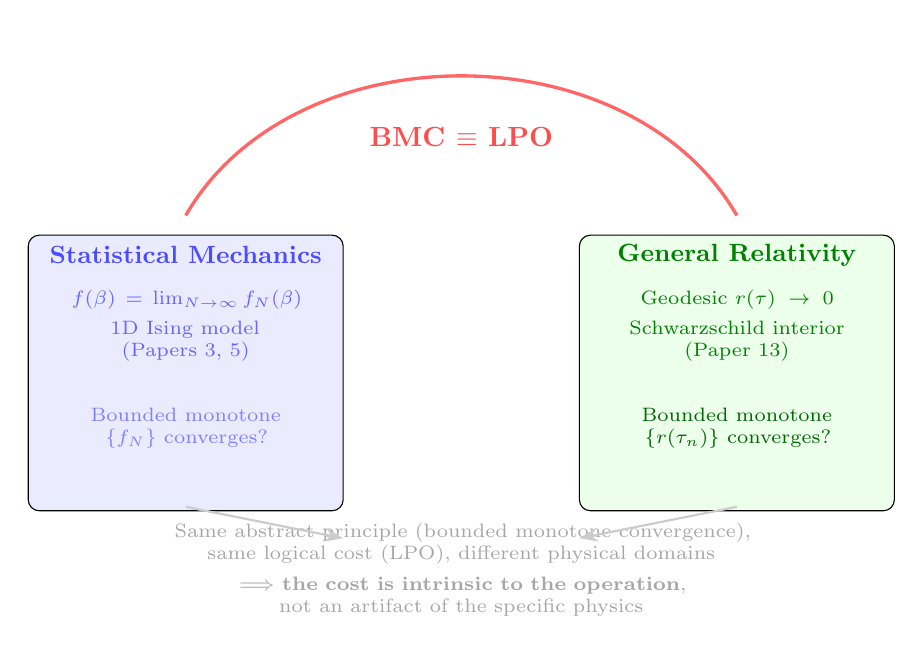
\begin{tikzpicture}[
  >=Stealth,
  every node/.style={font=\small},
  pillar/.style={draw, rounded corners, minimum width=4cm, minimum height=3.5cm, align=center, inner sep=6pt}
]
% Left pillar: Statistical Mechanics
\node[pillar, fill=blue!8] (sm) at (-3.5, 0) {};
\node[font=\small\bfseries, blue!70] at (-3.5, 1.5) {Statistical Mechanics};
\node[font=\scriptsize, blue!60, text width=3.5cm, align=center] at (-3.5, 0.6)
  {$f(\beta) = \lim_{N\to\infty} f_N(\beta)$\\[3pt]1D Ising model\\(Papers 3, 5)};
\node[font=\scriptsize, blue!50, text width=3.5cm, align=center] at (-3.5, -0.7)
  {Bounded monotone\\$\{f_N\}$ converges?};

% Right pillar: General Relativity
\node[pillar, fill=green!8] (gr) at (3.5, 0) {};
\node[font=\small\bfseries, green!50!black] at (3.5, 1.5) {General Relativity};
\node[font=\scriptsize, green!50!black, text width=3.5cm, align=center] at (3.5, 0.6)
  {Geodesic $r(\tau) \to 0$\\[3pt]Schwarzschild interior\\(Paper 13)};
\node[font=\scriptsize, green!40!black, text width=3.5cm, align=center] at (3.5, -0.7)
  {Bounded monotone\\$\{r(\tau_n)\}$ converges?};

% Bridge/arch
\draw[very thick, red!60] (-3.5, 2.0) to[out=60, in=120] (3.5, 2.0);
\node[font=\normalsize\bfseries, red!70, fill=white, inner sep=3pt] at (0, 3.0)
  {BMC $\equiv$ LPO};

% Below: explanation
\node[font=\scriptsize, gray!70, text width=8cm, align=center] at (0, -2.5)
  {Same abstract principle (bounded monotone convergence),\\
   same logical cost (LPO), different physical domains\\[3pt]
   $\Longrightarrow$ \textbf{the cost is intrinsic to the operation},\\
   not an artifact of the specific physics};

% Arrows down to explanation
\draw[->, thick, gray!40] (-3.5, -1.7) -- (-1.5, -2.1);
\draw[->, thick, gray!40] (3.5, -1.7) -- (1.5, -2.1);

\end{tikzpicture}
\caption{Domain invariance: the same logical cost in different physics.
The bounded monotone convergence equivalence (BMC~$\equiv$~LPO) appears
independently in statistical mechanics (thermodynamic limit) and general
relativity (geodesic incompleteness).
That the same abstract principle governs both is evidence that the logical
cost is intrinsic to the mathematical operation, not to the physical domain.}
\label{fig:domain-invariance}
\end{figure}

\begin{keymessage}
\textbf{Hypothesis:} empirical predictions are BISH-derivable; stronger logic enters only through idealizations no finite laboratory can instantiate.
This is not operationalism---it distinguishes physical content (BISH) from mathematical infrastructure (WLPO/LPO/LEM).
The non-constructive superstructure is not wrong; it is \emph{physically idle}.
\end{keymessage}

% ============================================================
\section{Objections and Open Problems}
% ============================================================

Intellectual honesty requires confronting the strongest objections.

\emph{``The constructive hierarchy tracks mathematical generality, not physical depth.''}
If the correlation between logical strength and idealization were merely a reflection of mathematical complexity---simple theorems are constructive, deep theorems are not---the hypothesis would be trivial.
But the correlation is between logical strength and \emph{physical accessibility}: whether a finite laboratory can instantiate the objects described.
The error bounds for the Ising model are mathematically non-trivial---they involve transfer matrix eigenvalues, logarithmic estimates, and geometric series analysis---but they are BISH because every object in the proof is finitely constructible.
The thermodynamic limit is mathematically elementary---it is just a limit of a monotone sequence---but it requires LPO because the limiting object is infinitely far from any finite approximation in a precise logical sense.
The hierarchy tracks physical accessibility, not mathematical sophistication.

\emph{``What about essential idealizations?''}
Batterman \cite{Batterman2005} has argued that infinite idealizations are ``explanatorily essential''---that the thermodynamic limit, for instance, is not merely a convenience but genuinely explains universality and critical phenomena in a way that finite-system descriptions do not.
Our results address \emph{predictive} content, not \emph{explanatory} content.
The finite-size error bounds reproduce every number a laboratory can measure.
Whether the \emph{explanatory power} of universality classes and critical exponents can be captured without the completed limit is an open question---one of the most important in the philosophy of physics \cite{vanWierst2019}.
We take no position on it here.

\emph{``Doesn't Dyson's divergence of the perturbation series undermine the claim that QED predictions are BISH?''}
No---the opposite.
The finite-order truncation \emph{is} the BISH content.
The divergence of the full series is an LPO-level statement about the cathedral: it asserts that a particular infinite object (the formal sum of all loop orders) fails to converge.
But the predictions come from the truncation, not the sum.
The fact that truncated perturbation theory produces the most precise predictions in physics is precisely the cellar-and-cathedral pattern: the cellar (finite-order Feynman diagrams) delivers the predictions; the cathedral (the infinite series, the path integral, the non-perturbative completion) organizes them.
Dyson's result shows that the cathedral is asymptotic, not convergent---which, if anything, strengthens the case that the physics lives in the cellar.
The justification for trusting the truncation---that the first $n$ terms of an asymptotic series approximate the true value with error bounded by the $(n{+}1)$th term---is itself a BISH-level finite error estimate, even though the asymptotic analysis that establishes this bound may invoke classical techniques.
In effective field theory, the truncation order is set by the energy scale and desired precision---a constructive criterion---not by convergence of the infinite series.

\emph{``Is formulation-invariance robust?''}
The formulation-invariance test---identical axiom profiles across two independent derivations \cite{Lee2026e}---is evidence, not proof.
Two formulations yielding the same logical cost is more compelling than one, but a definitive ineliminability theorem---proving that \emph{any} constructive proof of Ising free energy convergence must use LPO---remains open.

\emph{Open problems.}
Several questions that were open in v2.0 have been resolved.
The LLPO gap---``is there a physical statement whose logical cost is exactly LLPO?''---has been answered affirmatively three times over: WKB turning-point existence (Paper~19 \cite{Lee2026paper19}), Bell's disjunction (Paper~21 \cite{Lee2026paper21}), and Kochen-Specker contextuality (Paper~24 \cite{Lee2026paper24}) all cost exactly LLPO\@.
The Fan Theorem, previously absent from the calibration table, now has physical content: variational ground-state existence (Paper~23 \cite{Lee2026paper23}).

New questions replace the old ones.
What is the constructive cost of renormalization group flows in quantum field theory beyond the Yukawa sector (Paper~18)?
Can the GNS construction---the passage from abstract $C^*$-algebraic states to Hilbert space representations---be calibrated?
How does the D\"oring-Isham topos program \cite{DoeringIsham2008}, which arrives at intuitionistic logic through a completely different route, relate to the constructive hierarchy?
Is the observable-dependence of logical cost (Paper~20) a general phenomenon, or are there systems where every observable costs the same level?
Can the five-domain BMC~$\equiv$~LPO pattern be extended to quantum field theory---does the continuum limit of a lattice gauge theory cost exactly LPO?

And the deepest open problem of all: what is \emph{the principle}?
The calibration table establishes a correlation between logical strength and physical idealization.
A fully satisfying account would provide a single physical principle---analogous to the constancy of the speed of light or the equivalence principle---from which the correlation \emph{follows}.
Why BISH?
What is it about the physical world that makes constructive logic the right logic for empirical predictions?
No one has this principle.
Finding it would transform the correlation into a theorem and the hypothesis into a physical law.
Such a principle would be a physical postulate---analogous to ``no superluminal signaling'' or ``the equivalence of inertial frames''---from which BISH-derivability of empirical content follows as a consequence.
The calibration table constrains what such a principle can say; it does not yet say it.
It remains the most important open problem the research program has generated.

\begin{keymessage}
The hierarchy tracks physical accessibility, not mathematical sophistication.
The correlation between logical strength and idealization is robust but not yet explained by a single principle.
The deepest open problem: what physical principle explains why nature speaks the language of constructive logic?
\end{keymessage}

% ============================================================
\section{Return to the Cellar}
% ============================================================

Return to the anomalous magnetic moment of the electron.

The number that theory and experiment agree on, to twelve decimal places, is a BISH computation---constructive analysis, not merely finite arithmetic.
Finite Feynman diagrams, finite integrals, finite arithmetic.
No path integrals, no Fock space, no renormalization group fixed points.
The cathedral of infinite-dimensional mathematical physics sits above this number: beautiful, structurally impressive, useful as a mnemonic for organizing the computation.
And largely idle as far as empirical predictions are concerned.

The constructive hierarchy---developed by Brouwer for philosophical reasons, refined by Bishop \cite{Bishop1967} for mathematical reasons, and sharpened by Bridges, Ishihara \cite{Ishihara1992, Ishihara2006}, and their students into a precise instrument of logical calibration---turns out to be the right tool for mapping the boundary between the physical world and the mathematical structures we use to describe it.
It was not designed for this purpose.
It was designed to answer questions about the foundations of mathematics.
That it answers questions about the foundations of physics is either a coincidence or evidence that the questions are the same question.

Whether nature is constructive---whether the physical universe computes at BISH---is a hypothesis, not a theorem.
The evidence is growing: across quantum mechanics, statistical mechanics, general relativity, black hole thermodynamics, quantum field theory, and the foundations of quantum information, every empirical prediction we have checked lives at sea level, and the classical superstructure is scaffolding.
The hierarchy is a tree, not a chain: the omniscience spine has three populated intermediate levels (LLPO, WLPO, LPO), and three independent branches (DC$_\omega$, MP, FT) carry distinct physical content.
For the first time, this evidence is machine-verified: 18,500~lines of Lean~4 proofs with auditable axiom certificates, ensuring that the logical bookkeeping is exact.

The hypothesis could be wrong.
A single empirical prediction that provably requires LPO would refute it.
A physical phenomenon that lives genuinely at WLPO---whose operational content, not just its mathematical formulation, requires an omniscience principle---would force a revision.
The hypothesis is stated precisely enough to be falsifiable, which is all one can ask of a scientific proposal.

But if it is right, the implications extend beyond the calibration table.
The 150-year history of mathematical physics---from Weierstrass through Boltzmann, von~Neumann, Penrose, and the Standard Model---is a history of a community progressively importing logical strength while the operational content of its theories stayed at the most elementary level (Figure~\ref{fig:timeline}).
The tree structure of the hierarchy means the import happened along multiple independent axes simultaneously: omniscience (LPO) for limits, choice (DC$_\omega$) for measurement, compactness (FT) for variational principles, and sign-determination (LLPO) for disjunctions.
Each generation adopted a more powerful mathematical formalism, each formalism produced brilliant predictions, and nobody noticed that the predictions could have been extracted from a weaker logical base, because nobody had a tool for measuring logical strength with sufficient precision.

We now have the tool.
The calibration table is not the end of the story; it is the beginning.
It tells us where the map matches the territory and where the mapmaker's conventions begin.
What remains is the hardest part: not merely identifying the surplus structure, but understanding why it is surplus---finding the principle that explains why the physical world speaks the language of constructive logic, if indeed it does.

The most precise prediction in physics requires the least logical strength.
That may be the most important thing the prediction tells us.

% ============================================================
\appendix
\section{Why It Matters --- A Guide for the Working Physicist}
\label{app:why}

This appendix summarizes each paper in the series for readers unfamiliar with constructive mathematics. The key idea: when physicists use infinite idealizations (limits, completed real numbers, spectral decompositions), they are making specific logical commitments that go beyond what any finite experiment can verify. This programme identifies \emph{exactly which} commitment each idealization requires.

\medskip

\textbf{The hierarchy in one sentence.} BISH is what a computer can do; LLPO is deciding a sign; WLPO is deciding whether something is zero; LPO is deciding a yes/no question about an infinite sequence; MP is concluding existence from non-impossibility; FT is extracting a uniform bound from pointwise data; DC$_\omega$ is making infinitely many dependent choices.

\medskip

\textbf{Paper~2} (WLPO). When you write $\langle\psi|$ and treat it as living in the ``same'' space as $|\psi\rangle$, you are assuming WLPO\@. The gap between a space and its double dual is real and has a logical cost.

\textbf{Paper~4} (BISH to Undecidable). The spectrum of a quantum observable has five layers of logical difficulty, from ``approximate eigenvalues exist'' (trivial) to ``is the spectral gap zero?'' (unsolvable by any algorithm).

\textbf{Paper~5} (BISH). General relativity at any finite radius outside a black hole is fully constructive. Spacetime curvature is computable. The non-constructive problems start only when you extend geodesics to infinity or to singularities.

\textbf{Paper~6} (BISH). The Heisenberg uncertainty principle is just Cauchy--Schwarz. No deep logic, no observer effects, no non-constructive axioms. It is a theorem about geometry.

\textbf{Paper~7} (WLPO). Density matrices that cannot be represented by any physical state exist only with WLPO\@. The mathematical overhead of infinite-dimensional Hilbert spaces has a precise cost.

\textbf{Paper~8} (LPO). Every time you take a thermodynamic limit, you are making a specific logical commitment---LPO---that no finite experiment can verify. This is not a metaphor; it is a theorem. The Ising model proves it in both directions.

\textbf{Paper~9} (Methodology). It does not matter whether you derive the Ising model via transfer matrices or combinatorics. The logical cost is the same either way. The cost belongs to the physics, not the proof technique.

\textbf{Paper~11} (BISH). Quantum entanglement---including the Tsirelson bound, Bell state entropy, and the partial trace---is fully constructive. The ``spookiness'' of entanglement is computable; the logical cost enters only when you pass to infinite-dimensional systems.

\textbf{Paper~13} (LPO). The event horizon of a black hole is a logical boundary, not just a physical one. Inside and outside are both constructive. But asserting that the infalling trajectory \emph{reaches} the singularity requires LPO---the same principle as the thermodynamic limit. The deepest boundary in general relativity and the deepest boundary in constructive mathematics coincide.

\textbf{Paper~14} (LPO). Wave function collapse, formulated as the infinite-time limit of decoherence, costs LPO\@. The finite-time decoherence process is BISH\@. The ``mystery'' of collapse is a limit problem, not a quantum problem.

\textbf{Paper~15} (LPO). Noether's theorem in finite dimensions is BISH\@. But global energy conservation for infinite systems requires LPO\@. Interestingly, the sign of the energy density matters: non-negative gives you monotone sequences (LPO), signed gives you oscillations (harder).

\textbf{Paper~16} (DC$_\omega$). The measurement problem is not a physics problem. It is a disagreement about whether to accept dependent countable choice for the convergence of relative frequencies. Every finite set of measurement outcomes is constructive. The controversy lives entirely in the infinite limit.

\textbf{Paper~17} (LPO). Bekenstein--Hawking entropy is constructive for any finite discretization. But asserting that entropy per unit area converges to the Bekenstein--Hawking value costs LPO\@. Quantum gravity pays the same logical price as statistical mechanics.

\textbf{Paper~18} (BISH). A negative result that matters. The Standard Model's Yukawa RG evolution is entirely constructive. Removing the non-constructive scaffolding from the fermion mass problem reveals\ldots\ nothing new. The scaffolding is idle, but removing it does not solve the mass hierarchy.

\textbf{Paper~19} (LLPO). Quantum tunnelling through a specific barrier is constructive. But asserting that a \emph{general} continuous potential has classical turning points costs LLPO\@. The WKB approximation has three logical tiers, and the middle one---turning-point existence---is the first physical appearance of LLPO\@.

\textbf{Paper~20} (WLPO). The 1D Ising model's thermodynamic limit costs LPO (Paper~8). But just classifying its phase---asking ``is the magnetization zero or not?''---costs only WLPO\@. The logical price depends on the question, not just the system.

\textbf{Paper~21} (LLPO). Bell's theorem refutes local hidden variables constructively (BISH). But the physicist's conclusion---``either locality fails \emph{or} realism fails''---costs LLPO\@. The price of the \emph{or}.

\textbf{Paper~22} (MP). ``This nucleus is unstable, so it will eventually decay.'' That inference requires Markov's Principle. The tunnelling traversal time controversy is a disagreement about MP, not about physics.

\textbf{Paper~23} (FT). ``A continuous function on a compact set attains its minimum.'' Physicists use this constantly---in variational principles, ground state existence, equilibrium optimization. It requires the Fan Theorem, which is independent of every other principle in the hierarchy. Different types of mathematical reasoning draw on different logical wells.

\textbf{Paper~24} (LLPO). Kochen--Specker contextuality has exactly the same logical cost as Bell nonlocality: LLPO\@. Two physically unrelated impossibility theorems turn out to be the same logical phenomenon. Constructive mathematics sees what classical mathematics cannot.

\medskip

\textbf{The punchline.} Every empirical prediction in physics---every number that agrees with experiment---can be derived using only BISH, the weakest constructive logic. Stronger principles enter only through idealizations (infinite limits, completed reals, global existence claims) that no laboratory can instantiate. The calibration table tells you exactly which idealization carries which logical price. That distinction---between what nature requires and what the formalism demands---is the oldest question in philosophy of physics, and this programme gives it the first formally precise answer.


% ============================================================
\section{How the Programme Developed --- Four Phases of Discovery}
\label{app:development}
% ============================================================

Paper~10, \S6 traces the programme's intellectual development in full technical detail.
This appendix tells the same story in terms that connect directly to physics.
At each stage the driving question was: \emph{what is the logical price of the mathematical machinery physicists use?}

\bigskip

\textbf{Phase~1: ``Does the question have a non-trivial answer?''}

Physicists already suspect that infinite limits are ``more dangerous'' than finite calculations, but they have no formal vocabulary for saying \emph{how much} more dangerous. The first papers tested whether a formal vocabulary could be built.

Paper~2 examined bra-ket notation. Writing $\langle\psi|$ and treating it as living in the ``same'' space as $|\psi\rangle$ means identifying a Hilbert space $H$ with its double dual $H^{**}$. The logical cost: WLPO --- roughly, the ability to decide whether an infinite binary sequence is all zeros. Not the strongest non-constructive principle, but not free.

Paper~4 asked a harder question: how many logical layers does spectral theory have? The answer: at least five. Approximate eigenvalues are BISH (a computer can find them). Whether the spectral gap vanishes is undecidable (no algorithm can determine it in general). Between these extremes sit three more levels. Quantum mechanics is not a monolithic logical commitment; it is a layered structure, and each layer costs something different.

Paper~6 provided a welcome surprise. The Heisenberg uncertainty principle --- the Robertson-Schr\"odinger form that appears in every textbook --- is BISH: pure Cauchy-Schwarz geometry. No non-constructive axiom is needed. One of the most philosophically debated results in physics is, logically, among the cheapest.

At the end of Phase~1, the programme had proof of concept: the logical hierarchy has real content for physics. What it lacked was a \emph{technique}. Most of these early results were one-directional: ``Theorem~X \emph{requires} at least WLPO.'' The programme needed a clean two-directional equivalence to sharpen the picture.

\bigskip

\textbf{Phase~2: ``Is there a systematic pattern?''}

The breakthrough came with the 1D Ising model (Paper~8). Consider the simplest possible statistical-mechanical system: a chain of spins with nearest-neighbour coupling. The finite-volume free energy can be computed in BISH --- a straightforward matrix diagonalisation, no omniscience needed. But the thermodynamic limit --- the assertion that the free energy \emph{per site} converges to a definite real number as the chain length goes to infinity --- is \emph{equivalent} to LPO, the strongest omniscience principle below full classical logic. The equivalence is tight: LPO implies the limit exists, and the existence of the limit implies LPO. Both directions are proved, both are machine-verified.

The physical message: you can compute the free energy at any finite chain length to arbitrary precision without invoking LPO (the ``dispensability'' result of Part~A). The error decays exponentially with chain length. The thermodynamic limit is a mathematical convenience, not a physical necessity. The cathedral is beautiful, but the cellar is where the predictions live.

Then the same pattern appeared in completely different physics. Geodesic incompleteness in the Schwarzschild interior: LPO via BMC (Paper~13). Exact decoherence in the infinite-environment limit: LPO via a variant of BMC (Paper~14). Global energy existence from Noether's theorem: LPO via another BMC variant (Paper~15). Four independent domains of physics, one logical pattern. And the cost was formulation-invariant: rederiving the Ising free energy combinatorially instead of via transfer matrices gave the identical axiom profile (Paper~9). The logical cost belongs to the physics, not to the proof technique.

\bigskip

\textbf{Phase~3: ``How far does it go?''}

Papers~16, 17, and~18 asked whether CRM could illuminate genuinely open questions in physics.

Paper~16 addressed the measurement problem. Born probabilities --- the rule $p = |\langle\phi|\psi\rangle|^2$ --- are BISH. A computer can evaluate them. But the strong law of large numbers --- the assertion that relative frequencies \emph{converge} to the Born probabilities --- requires DC$_\omega$ (dependent countable choice). The interpretive controversy around quantum measurement is partly a disagreement about whether to accept this particular logical commitment. The finite Born rule is uncontroversial; the controversy starts where the infinite-frequency interpretation begins.

Paper~17 extended the programme to quantum gravity. The Bekenstein-Hawking formula $S = A/4$, as derived from loop quantum gravity state counting, follows the same BMC~$\equiv$~LPO pattern as the Ising model. The entropy density converges, but convergence costs LPO. A fifth independent domain now exhibited the pattern. At this point, dismissing the correlation as coincidence required increasingly strained special pleading.

Paper~18 defined the boundary. The fermion mass hierarchy --- why the top quark is $10^5$ times heavier than the electron --- consists of finite dimensionless ratios. These are already BISH. There is no finite/infinite stratification for CRM to exploit, and the Scaffolding Principle (removing non-constructive scaffolding to reveal new physics) produced nothing. This was a negative result, but a necessary one: it told us exactly what CRM \emph{cannot} do.

\bigskip

\textbf{Phase~4: ``What does the full picture look like?''}

The final phase addressed every gap in the hierarchy.

LLPO --- the principle that says ``this real number is non-negative or non-positive, but I cannot tell you which'' --- had no physical instantiation. Papers~19, 21, and~24 provided three. The WKB approximation in quantum tunnelling has a turning point where the potential crosses the energy level (Paper~19); deciding on which side of the crossing you stand costs LLPO. Bell's theorem says ``either locality fails or realism fails'' (Paper~21); this disjunction without constructive witness costs LLPO. Kochen-Specker contextuality says ``either non-contextual hidden variables fail or value-definiteness fails'' (Paper~24); same logical structure, same cost. All three are ``either A or B, but you cannot say which.''

The Bell-KS connection deserves emphasis. Physicists discuss Bell nonlocality and KS contextuality in different chapters of quantum foundations textbooks. One involves spatially separated systems; the other involves a single system. CRM revealed that they have \emph{exactly the same logical structure}: both are disjunctions without constructive witness, both cost LLPO, both for the same reason. Decades of informal analysis did not detect this identity. CRM did.

Paper~23 established the Fan Theorem as a third independent branch of the hierarchy. The extreme value theorem --- a continuous function on $[a,b]$ attains its maximum --- requires FT, which is independent of every other principle in the hierarchy. Convergence arguments (LPO), disjunction arguments (LLPO), and compactness arguments (FT) draw on different, mutually independent logical wells. The hierarchy is a tree, not a ladder.

Paper~20 returned to the 1D Ising model --- the programme's Rosetta Stone --- and discovered observable-dependent logical cost. The same system costs BISH (finite-volume bounds), WLPO (phase classification via magnetisation zero-test), LPO (thermodynamic limit), or FT (parameter-space optimisation), depending on which question is asked. Logical cost classifies \emph{questions}, not systems.

Paper~22 provided the programme's most striking diagnostic result. The tunnelling traversal time controversy --- a genuine, unresolved disagreement among physicists about whether quantum tunnelling takes a definite finite time --- was identified as a disagreement about Markov's Principle. The different positions in the debate correspond, precisely, to different commitments about whether double-negation existence (``it is not the case that the particle never arrives'') implies constructive existence (``the particle eventually arrives''). CRM did not resolve the physics; it clarified what the disagreement is actually about.

\bigskip

\textbf{Where this leaves us.} The programme began by asking whether the constructive hierarchy had anything to say about physics. It ended by detecting hidden structural identities, diagnosing genuine physical controversies, and revealing that the logical geography of mathematical physics is a tree with three independent branches --- each capturing a different mode of reasoning about the physical world. Whether this pattern reflects something about the logical structure of physical reality, or whether it is merely an artifact of the mathematical formalism physicists happen to use, is the question that connects all nineteen papers. It is also, arguably, the oldest question in philosophy of physics: what in our theories is about nature, and what is about us?

% ============================================================
\begin{thebibliography}{99}

\bibitem{Batterman2005}
R.~W.~Batterman,
``Critical phenomena and breaking drops: infinite idealizations in physics,''
\emph{Studies in History and Philosophy of Modern Physics} \textbf{36} (2005), 225--244.

\bibitem{Bishop1967}
E.~Bishop,
\emph{Foundations of Constructive Analysis},
McGraw-Hill, New York, 1967.

\bibitem{BridgesRichman1987}
D.~Bridges and F.~Richman,
\emph{Varieties of Constructive Mathematics},
Cambridge University Press, 1987.

\bibitem{BridgesVita2006}
D.~Bridges and L.~S.~V\^{\i}\c{t}\u{a},
\emph{Techniques of Constructive Analysis},
Springer, New York, 2006.

\bibitem{Cubitt2015}
T.~S.~Cubitt, D.~Perez-Garcia, and M.~M.~Wolf,
``Undecidability of the spectral gap,''
\emph{Nature} \textbf{528} (2015), 207--211.

\bibitem{DoeringIsham2008}
A.~D\"oring and C.~J.~Isham,
``\,`What is a thing?': Topos theory in the foundations of physics,''
in \emph{New Structures for Physics}, Lecture Notes in Physics \textbf{813}, Springer, 2008.

\bibitem{Dyson1952}
F.~J.~Dyson,
``Divergence of perturbation theory in quantum electrodynamics,''
\emph{Physical Review} \textbf{85}(4) (1952), 631--632.

\bibitem{Einstein1939}
A.~Einstein,
``On a stationary system with spherical symmetry consisting of many gravitating masses,''
\emph{Annals of Mathematics} \textbf{40} (1939), 922--936.

\bibitem{JNVWY2021}
Z.~Ji, A.~Natarajan, T.~Vidick, J.~Wright, and H.~Yuen,
``{MIP}$^*$ = {RE},''
\emph{Communications of the ACM} \textbf{64}(11) (2021), 131--138.

\bibitem{Gisin2020}
N.~Gisin,
``Mathematical languages shape our understanding of time in physics,''
\emph{Nature Physics} \textbf{16} (2020), 114--116.

\bibitem{Gisin2021}
N.~Gisin,
``Indeterminism in physics, classical chaos and Bohmian mechanics: Are real numbers really real?''
\emph{Erkenntnis} \textbf{86} (2021), 1469--1481.

\bibitem{GlimmJaffe1981}
J.~Glimm and A.~Jaffe,
\emph{Quantum Physics: A Functional Integral Point of View},
Springer, New York, 1981.

\bibitem{Haag1996}
R.~Haag,
\emph{Local Quantum Physics: Fields, Particles, Algebras},
2nd ed., Springer, Berlin, 1996.

\bibitem{Ishihara1992}
H.~Ishihara,
``Continuity properties in constructive mathematics,''
\emph{Journal of Symbolic Logic} \textbf{57} (1992), 557--565.

\bibitem{Ishihara2006}
H.~Ishihara,
``Reverse mathematics in Bishop's constructive mathematics,''
\emph{Philosophia Scientiae}, Cahier sp\'ecial \textbf{6} (2006), 43--59.

\bibitem{Kerr2023}
R.~P.~Kerr,
``Do black holes have singularities?''
Preprint, arXiv:2312.00841, 2023.

\bibitem{Lee2026a}
P.~C.-K.~Lee,
``Constructive reverse mathematics of the bidual gap: WLPO equivalence for Banach space non-reflexivity,''
2026. Zenodo DOI: 10.5281/zenodo.17107493.

\bibitem{Lee2026b}
P.~C.-K.~Lee,
``The physical bidual gap: WLPO and non-reflexivity of trace-class operators,''
2026. Zenodo DOI: 10.5281/zenodo.18509795.

\bibitem{Lee2026c}
P.~C.-K.~Lee,
``The constructive cost of the thermodynamic limit: LPO equivalence and BISH dispensability in the 1D Ising model,''
2026. Zenodo DOI: 10.5281/zenodo.18516813.

\bibitem{Lee2026e}
P.~C.-K.~Lee,
``Formulation-invariance of the logical cost of the thermodynamic limit: a combinatorial proof for the 1D Ising model,''
2026. Zenodo DOI: 10.5281/zenodo.18517570.

\bibitem{Lee2026f}
P.~C.-K.~Lee,
``Axiom calibration for quantum spectra: orthogonal heights, choice principles, and separation portals,''
2026. Zenodo DOI: 10.5281/zenodo.17059483.

\bibitem{Lee2026g}
P.~C.-K.~Lee,
``Constructive reverse mathematics for the Heisenberg uncertainty principle: Robertson-Schr\"odinger and Schr\"odinger inequalities over Mathlib,''
2026. Zenodo DOI: 10.5281/zenodo.18519836.

\bibitem{Lee2026paper10}
P.~C.-K.~Lee,
``The logical geography of mathematical physics: constructive calibration from density matrices to the event horizon,''
2026. Zenodo DOI: 10.5281/zenodo.18527559.

\bibitem{Lee2026paper11}
P.~C.-K.~Lee,
``Constructive entanglement: CHSH, Tsirelson bound, and Bell state entropy at BISH,''
2026. Zenodo DOI: 10.5281/zenodo.18527676.

\bibitem{Lee2026paper13}
P.~C.-K.~Lee,
``The event horizon as a logical boundary: Schwarzschild interior geodesic incompleteness and LPO in Lean~4,''
2026. Preprint. Paper~13 in the CRM series.

\bibitem{Lee2026paper14}
P.~C.-K.~Lee,
``Wave function collapse as a constructive limit: decoherence, LPO, and the infinite-time boundary,''
2026. Preprint. Paper~14 in the CRM series.

\bibitem{Lee2026paper15}
P.~C.-K.~Lee,
``Noether's theorem and the constructive cost of global conservation: finite symmetries at BISH, infinite systems at LPO,''
2026. Preprint. Paper~15 in the CRM series.

\bibitem{Lee2026paper16}
P.~C.-K.~Lee,
``The measurement problem as dependent choice: Born rule convergence and DC$_\omega$ in constructive quantum mechanics,''
2026. Preprint. Paper~16 in the CRM series.

\bibitem{Lee2026paper17}
P.~C.-K.~Lee,
``Bekenstein--Hawking entropy and the fifth BMC domain: constructive calibration of black hole thermodynamics,''
2026. Preprint. Paper~17 in the CRM series.

\bibitem{Lee2026paper18}
P.~C.-K.~Lee,
``The Scaffolding Principle: Yukawa RG evolution at BISH and the persistence of the fermion mass hierarchy,''
2026. Preprint. Paper~18 in the CRM series.

\bibitem{Lee2026paper19}
P.~C.-K.~Lee,
``LLPO and the WKB approximation: turning-point existence as the first physical appearance of the Lesser Limited Principle of Omniscience,''
2026. Preprint. Paper~19 in the CRM series.

\bibitem{Lee2026paper20}
P.~C.-K.~Lee,
``Observable-dependent cost: phase classification of the 1D Ising model at WLPO,''
2026. Preprint. Paper~20 in the CRM series.

\bibitem{Lee2026paper21}
P.~C.-K.~Lee,
``Bell's disjunction costs LLPO: constructive reverse mathematics of nonlocality,''
2026. Preprint. Paper~21 in the CRM series.

\bibitem{Lee2026paper22}
P.~C.-K.~Lee,
``Markov's Principle and the tunnelling traversal time: radioactive decay as a constructive inference,''
2026. Preprint. Paper~22 in the CRM series.

\bibitem{Lee2026paper23}
P.~C.-K.~Lee,
``The Fan Theorem in physics: variational minima, ground-state existence, and an independent branch of the hierarchy,''
2026. Preprint. Paper~23 in the CRM series.

\bibitem{Lee2026paper24}
P.~C.-K.~Lee,
``Kochen--Specker contextuality at LLPO: the same logical cost as Bell nonlocality,''
2026. Preprint. Paper~24 in the CRM series.

\bibitem{OppenheimerSnyder1939}
J.~R.~Oppenheimer and H.~Snyder,
``On continued gravitational contraction,''
\emph{Physical Review} \textbf{56} (1939), 455--459.

\bibitem{Penrose1965}
R.~Penrose,
``Gravitational collapse and space-time singularities,''
\emph{Physical Review Letters} \textbf{14}(3) (1965), 57--59.

\bibitem{Raychaudhuri1955}
A.~K.~Raychaudhuri,
``Relativistic cosmology.~I,''
\emph{Physical Review} \textbf{98} (1955), 1123--1126.

\bibitem{Redei1996}
M.~R\'edei,
``Why John von Neumann did not like the Hilbert space formalism of quantum mechanics (and what he liked instead),''
\emph{Studies in History and Philosophy of Modern Physics} \textbf{27}(4) (1996), 493--510.

\bibitem{vanDalen2005}
D.~van~Dalen,
\emph{Mystic, Geometer, and Intuitionist: The Life of L.~E.~J.~Brouwer}, Vol.~2,
Clarendon Press, Oxford, 2005.

\bibitem{vanWierst2019}
P.~van~Wierst,
``The paradox of phase transitions in the light of constructive mathematics,''
\emph{Synthese} \textbf{196} (2019), 1863--1884.

\bibitem{vonNeumann1932}
J.~von~Neumann,
\emph{Mathematische Grundlagen der Quantenmechanik},
Springer, Berlin, 1932.

\bibitem{Weyl1918}
H.~Weyl,
\emph{Das Kontinuum: Kritische Untersuchungen \"uber die Grundlagen der Analysis},
Veit, Leipzig, 1918.

\bibitem{Wilson1974}
K.~G.~Wilson,
``Confinement of quarks,''
\emph{Physical Review D} \textbf{10}(8) (1974), 2445--2459.

\end{thebibliography}

\bigskip
\section*{Statement of AI Use}

This essay was written with the assistance of Anthropic's Claude Opus~4.6.
The author's primary training is in interventional cardiology, not mathematical logic or mathematical physics; his main research interests are in applicational AI and medicine.
The formal results described herein are machine-verified in Lean~4, which is precisely the tool that decouples the validity of the proofs from the credentials of the prover.
The expository narrative should be read with this context in mind.

\end{document}
